\documentclass[12pt, a4paper]{article}
\usepackage{styles}

\begin{document}

% ====================  Deckblatt  ======================

    \begin{titlepage}


    \begin{figure}[h]
        \centering
        \begin{minipage}{0.30\textwidth}
            \centering
            
\includegraphics[width=\textwidth]{images/logo/parcit-logo.png}
        \end{minipage}
        \hspace{0.25\textwidth}
        \begin{minipage}{0.30\textwidth}
            \centering
            
\includegraphics[width=\textwidth]{images/logo/fh-aachen-logo.png}
        \end{minipage}
    \end{figure}

    \vspace{2cm}

    \begin{minipage}{0.9\textwidth}
        \fontsize{20pt}{16pt}\selectfont
        \begin{center}
            \textbf{Bachelor's Thesis}
        \end{center}
    \end{minipage}

    \vspace{0.5cm}

    \begin{minipage}{0.9\textwidth}
        \fontsize{14pt}{16pt}\selectfont
        \begin{center}
            in the Bachelor's Program 'Applied Mathematics and Computer Science'
        \end{center}
    \end{minipage}

    \vspace{2cm}

    \begin{minipage}{0.9\textwidth}
        \fontsize{20pt}{16pt}\selectfont
        \begin{center}
            \textbf{Backtesting and Live-Testing of Classic and AI-Powered Trading Strategies}
        \end{center}
    \end{minipage}


    \vspace{2cm}

    \begin{minipage}{0.9\textwidth}
        \fontsize{14pt}{16pt}\selectfont
        \begin{center}
            by
        \end{center}
    \end{minipage}

    \vspace{0.2cm}

    \begin{minipage}{0.9\textwidth}
        \fontsize{14pt}{16pt}\selectfont
        \begin{center}
            \textbf{Jason Becker}
        \end{center}
    \end{minipage}

    \vspace{0.2cm}

    \begin{minipage}{0.9\textwidth}
        \fontsize{14pt}{16pt}\selectfont
        \begin{center}
            Enrollment Number: 3567285
        \end{center}
    \end{minipage}

    \vspace{5cm}

    \begin{minipage}{0.9\textwidth}
        \fontsize{12pt}{16pt}\selectfont
        Supervisor: \ \ \ \ \ \ \ \ Prof. Dr. Bodo Kraft \\
        Co-Supervisor: \ \ \ Hendrik Karwanni, M. Sc. \\
        Submitted on: \ \ \ \ \today
    \end{minipage}

\end{titlepage}


    \newpage

    \newpage

    \pagestyle{empty}

\section*{Declaration of Authorship}

This bachelor thesis has been written by:

\begin{center}

    \textbf{Jason Becker} \\
    \textbf{Wachtelstraße 24} \\
    \textbf{40789 Monheim am Rhein}

\end{center}


\noindent
I hereby declare that this bachelor thesis has been written independently and without unauthorized assistance.
I confirm that I have used only the sources and aids indicated in the bibliography.
Furthermore, I declare that I have marked all passages that are either verbatim or paraphrased versions of sources.

I am aware that any form of plagiarism or dishonesty in academic work constitutes a serious offense and may lead to disciplinary measures.

\vspace{1cm}

\begin{flushright}
    \textbf{Monheim am Rhein, \today} \\
    \vspace{1.5cm}
    \textbf{......................................} \\
    \textbf{Jason Becker} \\
\end{flushright}

    \newpage

% ====================  Abstract  ======================


    \fancyfoot[C]{}
\vspace{0.7cm}

\section*{Abstract}

\vspace{0.5cm}

This bachelor's thesis examines the effectiveness of classical and AI-based algorithmic trading strategies using the ETH/USDC cryptocurrency pair on a per-minute basis (M1).
The goal is to improve informed trading decisions through data-driven methods.
The special feature of this currency pair lies in the combination of the high liquidity and volatility of ETH with the stability of USDC, which brings both advantages and disadvantages.


Therefore, a complete workflow is presented, from data acquisition via a broker API to feature engineering, the identification of market regimes, and the development and training of various deep learning models (FNN, LSTM, CNN, hybrid models), all the way to implementation and evaluation.

In addition to classic technical indicators such as moving averages and Bollinger Bands, AI-based regression and classification strategies were also developed and compared.
After retrieving the market data via the broker API, systematic feature engineering was performed, using not only traditional price- and volume-based indicators but also technical oscillators such as the RSI and MACD.
Principal component analysis (PCA) was also applied to reduce the dimensionality of the data and eliminate redundant information.


The Optuna framework, based on Bayesian optimization and enabling efficient hyperparameter search, was used to optimize the model parameters.
A dedicated loss function was implemented for the regression models, taking into account the practical application of the models in a trading context during training.


A particular focus of this work is the technical implementation of a modular trading engine.
The architecture of this engine allows the dynamic import and exchange of trading strategies, efficient processing of historical data, and both backtesting and live trading with real broker integration.
The implementation includes essential components such as an order execution module and data source modules that enable livestreaming of data via a broker or local loading of data, for example via CSV files.


To ensure realistic evaluation, the developed strategies were first optimized through backtests on historical data.
After identifying the best parameters, the most promising strategies were evaluated through out-of-sample tests, and one strategy was then deployed in a controlled live test with a real broker under actual market conditions.
During both development and live testing, various risk and money management concepts were applied to ensure capital preservation and controlled risk limitation.


The results show that both classical and AI-based approaches have their strengths.
However, the various strategies were severely affected by overfitting.
This was demonstrated by the fact that the strategies achieved profitable results on the data used for parameter selection but failed on previously unused test data.
This highlights the challenge of developing robust, generalizable strategies.
For this reason, a workflow was presented which could help to avoid overfitting in the development of trading strategies.
Although none of the tested strategies proved profitable in the long term, this work provides valuable insights into the relationship between AI and algorithmic trading, the importance of risk control, and the implementation of a fully automated trading system with direct connectivity to real brokers.




    \newpage

% ====================  Inhaltsverzeichniss  ======================
    \pagestyle{plain}
    \pagenumbering{roman}

    \tableofcontents

    \newpage


% ====================  Listings  ======================

    \pagenumbering{alph}

    \newpage
    \listoffigures


    \vspace{1.5cm}

    \listoftables


    \newpage
    \renewcommand{\thelstlisting}{\Alph{lstlisting}} % Code-Listings benuzen A, B, C, ...
    \lstlistoflistings

    \vspace{1.5cm}

    \section*{List of Abbreviations}

% Tabelle für das Abkürzungsverzeichnis
\begin{tabularx}{\textwidth}{@{}lL{0.8\textwidth}@{}}
    \textbf{ETH}  & Ethereum                              \\
    \textbf{BTC}  & Bitcoin                               \\
    \textbf{USDC} & USD Coin                              \\
    \textbf{DeFi}   & Decentralized Finance                 \\
    \textbf{M1}   & Minute-Level                          \\
    \textbf{OHLCV}  & Open, High, Low, Close, Volume        \\


    \textbf{PnL}  & Profit and Loss                       \\
    \textbf{TA}   & Technical Analysis                    \\
    \textbf{CFD}  & Contract For Difference               \\
    \textbf{EMA}  & Exponential Moving Average            \\
    \textbf{SMA}  & Simple Moving Average                 \\
    \textbf{MACD} & Moving Average Convergence/Divergence \\
    \textbf{ATR}  & Average True Range                    \\
    \textbf{TR}   & True Range                            \\
    \textbf{RSI}  & Relative Strength Index               \\
    \textbf{RRR}  & Risk-Reward Ratio                     \\
    \textbf{DD}   & Drawdown                              \\
    \textbf{MDD}  & Maximum Drawdown                      \\

    \textbf{PCA}  & Principal Component Analysis          \\
    \textbf{AI}   & Artificial Intelligence               \\
    \textbf{ML}     & Machine Learning                      \\
    \textbf{MLP}  & Multilayer Perceptron                 \\
    \textbf{FNN}  & Feedforward Neural Network            \\
    \textbf{RNN}  & Recurrent Neural Network              \\
    \textbf{GRU}  & Gated Recurrent Unit                  \\
    \textbf{LSTM} & Long Short-Term Memory                \\
    \textbf{CNN}  & Convolutional Neural Network          \\
    \textbf{ReLU} & Rectified Linear Unit                 \\
    \textbf{1D}   & One Dimensional                       \\
    \textbf{Conv1D} & Convolutional 1D                      \\

    \textbf{SPI}  & Service Provider Interface            \\
    \textbf{JAR}  & Java Archive                          \\
    \textbf{API}  & Application Programming Interface     \\

    \textbf{Min}  & Minimum                               \\
    \textbf{Max}  & Maximum                               \\
    \textbf{No}   & Number                                \\
    \textbf{UTC}  & Coordinated Universal Time            \\
    \textbf{PM}   & Post Meridiem                         \\
\end{tabularx}

    \newpage



    \pagenumbering{arabic}

    \section{Introduction}

\subsection{Motivation}

In recent years, the cryptocurrency market has emerged as a highly dynamic and rapidly evolving financial ecosystem.
Trading pairs such as \ethusdc on minute-level (M1) intervals provide vast amounts of high-frequency data, reflecting extreme volatility and market shifts.
This creates challenges and opportunities for traders and researchers.

The availability of detailed tick and minute data, combined with direct API access from crypto brokers, creates new opportunities for developing data-driven trading systems.
Advances in machine learning and deep learning offer promising tools to identify patterns in market movements.
This motivates an exploration of AI-based trading systems specifically designed for the \ethusdc pair, aiming to leverage technical features and advanced models to improve performance in the volatile cryptocurrency environment.

On the other hand, classical trading strategies also could perform well in this environment, especially if the strategies are adapted to specific market regimes.
Techniques such as moving averages, Bollinger Bands, or momentum indicators have the advantage of simplicity and transparency, allowing traders to understand and trust their decision-making process.

The ETH/USDC trading pair at the minute timescale was deliberately chosen because it offers several key advantages for analyzing and modeling algorithmic trading strategies.
Ethereum is one of the largest and most liquid cryptocurrencies in the world, while USDC, as a stablecoin, is subject to lower price fluctuations.
This combination allows for a clear separation between the volatile component (ETH) and a stable reference currency (USDC), simplifying analysis.
The high liquidity of this pair also ensures a reliable data basis with low slippage and tight spreads.
In particular, the M1 timescale provides sufficiently granular information to identify short-term market movements and micro-patterns without completely relying on high-frequency tick data.
This creates a practical scenario for the development and evaluation of trading algorithms that are both data-driven and operationally realistic.


\subsection{Aim of this Paper}

The primary goal of this paper is to develop and evaluate AI-powered and classical trading strategies focused on the \ethusdc cryptocurrency pair.
This paper will:

\begin{enumerate}
    \item Retrieve historical \ethusdc data via a broker API and process it for analysis.
    \item Perform exploratory data analysis and feature engineering, including trend, volatility, and momentum indicators.
    \item Identify and classify distinct market regimes to provide adaptive trading decisions.
    \item Apply risk and money management techniques to realistically simulate trading performance.
    \item Design, train, and benchmark multiple deep learning architectures such as LSTM, CNN, and hybrid models for forecasting the price and classify trading decisions.
    \item Develop algorithmic trading strategies based on AI model predictions and compare them with classical technical trading approaches.
    \item Build a modular trading engine capable of backtesting trading strategies and live execution using real broker connections.
    \item Execution of the final best trading strategy in live operation on a demo account with a real broker.
\end{enumerate}

\noindent
By focusing on the \ethusdc pair, this paper aims to provide insights into the effectiveness of deep learning and classical strategies in cryptocurrency trading and contribute practical tools for automated, adaptive trading in this challenging asset class.


    \newpage

    \section{Data Source and Broker Selection}

Cryptocurrency brokers (also called crypto brokers) play an important role in cryptocurrency trading.
Among other things, they act as intermediaries between different market participants.
Their key tasks include:

\begin{enumerate}
    \item \textbf{Providing access:} Individuals can participate in the market through a broker and thereby trade various cryptocurrencies.
    This includes executing orders such as buying cryptocurrencies at the lowest available price or selling them at the highest available price.
    \item \textbf{Security, and Compliance:} They also provide customers with a secure platform for executing transactions and adhere to the financial regulations established by authorities.
    \item \textbf{Leveraging:} Brokers offer customers the opportunity to borrow money, and thus trade with more capital than they actually have in their account.
\end{enumerate}


This has the advantage that trading with cryptocurrencies is much easier and safer, but one of the biggest disadvantages is the fees that are incurred when using \cite{broker-investing}.

\subsection{Broker Selection}
\label{chap:broker-selection}

For this paper, one broker must be selected for data retrieval and live testing.
Since the process is fully automated in short time-frames, the broker must meet certain requirements.

The API must be able to stream market data, request historical data, the current account balance, closed trades, and currently open positions, placing orders, and positions, as well as canceling unfilled orders.

Apart from the API, the broker must support leveraged long/short products like CFDs or margin trading.
They also must provide data in high quality as well as a demo depot.
The further they must be regulated in the European Union with the lowest possible fees.

\autoref{tbl:broker-comparision} summarizes the required features for some potential brokers.
All listed there meet the API functionality requirements.\footnote{Sources: \cite{bybit-home}, \cite{bybit-api-doc}, \cite{ig-home}, \cite{ig-api-doc}, \cite{capital-home}, \cite{capital-api-doc}}

\begin{table}[H]
    \small
    \centering
    \begin{tabular}{L{2cm} P{3.5cm} c c P{2cm}}
        \toprule
        Broker & Tradable assets & \multicolumn{2}{c}{\makecell{Fees}} & Leverage \\
        &                                            & Maker  & Taker   &      \\
        \midrule
        \textbf{ByBit} & Spot, Spot with leverage, Futures, Options & 0.02\% & 0.055\% & 10:1 \\
        \addlinespace[0.8em]
        \textbf{IG} & CFDs, Knock-out-Options & \multicolumn{2}{c}{Spread (approx.
        \$1.30)} & 2:1 \\
        \addlinespace[0.8em]
        \textbf{Capital.com} & CFDs & \multicolumn{2}{c}{Spread (approx.
        \$1.75)} & 2:1 \\
        \bottomrule
    \end{tabular}
    \caption{Broker Comparison}
    \label{tbl:broker-comparision}
\end{table}


Taking into account \autoref{tbl:broker-comparision}, ByBit is the best broker because it has the lowest fees, high quality data, the highest possible leverage as well as a regularization in the EU.

\subsection{API Connection and Data Retrieval Process}

Before starting with the Machine Learning process, and the backtests, the first step is to download historical \ethusdc via the ByBit API.
The request was executed on the \texttt{/v5/market/kline} API-Endpoint \cite{bybit-api-doc-get-kline} with the category \verb|linear|, symbol \verb|ETHPERP|, and interval \verb|1| at \ethDataEndDate.
Since ByBit only returns 1000 candlesticks per request, the same request with different start-, and end-times was executed until the ByBit API does no longer return older candlestick data.
This resulted in a candlestick data pool with data on a minute basis from \ethDataStartDate to \ethDataEndDate.
Chapter \ref{chap:statistics} will go into more detail about the data.

    \newpage

    \section{Exploratory Data Analysis}

\subsection{Statistics}
\label{chap:statistics}

\subsection{Dividing the Data}

Unlike classic machine learning processes, where data is splitted in three subsets, named train-, validation-, and test-set, here the data is splitted in four subsets. The fourth data-set is used for backtesting the real trading strategy, and is therefore not part of the machine learning process but plays an important role in developing the final trading strategy.

\begin{table}[H]
    \centering
    \begin{tabular}{ L{1.5cm} >{\centering\arraybackslash}m{4cm} >{\centering\arraybackslash}m{2cm} P{2.5cm} P{1.5cm} }
        \toprule
        Set & From & To & No. of Datapoints & \% of All Data
        \\
        \midrule
        \textbf{Complete} & \makecell{08/05/2022 \\ 10:00 UTC+2} & \makecell{06/17/2025 \\ 11:30 UTC+2} & $1,507,598$ & \\
        \addlinespace[0.8em]
        \textbf{Train} & \makecell{08/05/2022 \\ 10:00 UTC+2} & \makecell{04/30/2024 \\ 23:59 UTC+2} & $913,684$ & $60.6\%$ \\
        \addlinespace[0.8em]
        \textbf{Validation} & \makecell{05/01/2024 \\ 00:00 UTC+2} & \makecell{09/30/2024 \\ 23:59 UTC+2} & $220,320$ & $14.6\%$ \\
        \addlinespace[0.8em]
        \textbf{Test} & \makecell{10/01/2024 \\ 00:00 UTC+2} & \makecell{12/31/2024 \\ 23:59 UTC+2} & $132,482$ & $8.8\%$ \\
        \addlinespace[0.8em]
        \textbf{Backtest} & \makecell{01/01/2025 \\ 00:00 UTC+2} & \makecell{06/17/2025 \\ 11:30 UTC+2} & $241,111$ & $15.9\%$ \\
        \addlinespace[0.8em]
        \bottomrule
    \end{tabular}
    \caption{Data Split}
    \label{tbl:data-split}
\end{table}

After the splitting, the four subsets have the following summaries:

\begin{table}[H]
    \centering
    \begin{tabular}{cccccc}
        \toprule
        & Open & High & Low & Close & Volume
        \\
        \midrule
        & Open & High & Low & Close & Volume
        \\
        \textbf{count} & 913684.0 & 913684.0 & 913684.0 & 913684.0 & 913684.0 \\
        \textbf{mean}  & 1933.4   & 1933.95  & 1932.85  & 1933.4   & 7.58     \\
        \textbf{std}   & 619.6    & 619.92   & 619.28   & 619.6    & 105.09   \\
        \textbf{min}   & 1074.35  & 1077.45  & 1064.05  & 1074.35  & 0.0      \\
        \textbf{25\%}  & 1578.44  & 1578.89  & 1577.99  & 1578.44  & 0.0      \\
        \textbf{50\%}  & 1801.52  & 1801.81  & 1801.13  & 1801.52  & 0.05     \\
        \textbf{75\%}  & 2083.4   & 2083.84  & 2083.05  & 2083.4   & 2.02     \\
        \textbf{max}   & 4098.5   & 4099.48  & 4096.35  & 4098.5   & 31350.65 \\
        \bottomrule
    \end{tabular}
    \caption{Train Data}
    \label{tbl:train-data}
\end{table}

\begin{table}[H]
    \centering
    \begin{tabular}{cccccc}
        \toprule
        & Open & High & Low & Close & Volume
        \\
        \midrule
        \textbf{count} & 220320.0 & 220320.0 & 220320.0 & 220320.0 & 220320.0 \\
        \textbf{mean}  & 3050.36  & 3051.3   & 3049.4   & 3050.36  & 2.89     \\
        \textbf{std}   & 473.4    & 473.45   & 473.34   & 473.4    & 21.45    \\
        \textbf{min}   & 2111.8   & 2160.4   & 2088.13  & 2111.8   & 0.0      \\
        \textbf{25\%}  & 2617.31  & 2618.04  & 2616.71  & 2617.31  & 0.0      \\
        \textbf{50\%}  & 3063.4   & 3064.31  & 3062.43  & 3063.4   & 0.12     \\
        \textbf{75\%}  & 3462.22  & 3463.29  & 3461.21  & 3462.22  & 1.32     \\
        \textbf{max}   & 3974.68  & 3976.96  & 3969.94  & 3974.68  & 4972.18  \\
        \bottomrule
    \end{tabular}
    \caption{Validation Data}
    \label{tbl:validation-data}
\end{table}

\begin{table}[H]
    \centering
    \begin{tabular}{cccccc}
        \toprule
        & Open & High & Low & Close & Volume
        \\
        \midrule
        \textbf{count} & 132482.0 & 132482.0 & 132482.0 & 132482.0 & 132482.0 \\
        \textbf{mean}  & 3093.93  & 3095.27  & 3092.58  & 3093.94  & 4.42     \\
        \textbf{std}   & 531.85   & 532.29   & 531.4    & 531.85   & 18.42    \\
        \textbf{min}   & 2309.01  & 2311.73  & 2307.73  & 2309.01  & 0.0      \\
        \textbf{25\%}  & 2541.8   & 2542.65  & 2540.94  & 2541.8   & 0.08     \\
        \textbf{50\%}  & 3143.69  & 3145.38  & 3142.02  & 3143.7   & 0.68     \\
        \textbf{75\%}  & 3487.9   & 3489.46  & 3486.33  & 3487.9   & 2.92     \\
        \textbf{max}   & 4107.28  & 4112.68  & 4102.6   & 4107.28  & 1341.05  \\
        \bottomrule
    \end{tabular}
    \caption{Test Data}
    \label{tbl:test-data}
\end{table}

\begin{table}[H]
    \centering
    \begin{tabular}{cccccc}
        \toprule
        & Open & High & Low & Close & Volume
        \\
        \midrule
        \textbf{count} & 241111.0 & 241111.0 & 241111.0 & 241111.0 & 241111.0 \\
        \textbf{mean}  & 2432.57  & 2433.77  & 2431.35  & 2432.57  & 7.0      \\
        \textbf{std}   & 574.72   & 574.95   & 574.49   & 574.72   & 32.11    \\
        \textbf{min}   & 1386.6   & 1395.8   & 1382.99  & 1386.6   & 0.0      \\
        \textbf{25\%}  & 1887.22  & 1888.28  & 1886.1   & 1887.22  & 0.18     \\
        \textbf{50\%}  & 2510.29  & 2511.4   & 2509.1   & 2510.29  & 1.26     \\
        \textbf{75\%}  & 2732.0   & 2733.21  & 2730.7   & 2732.0   & 4.94     \\
        \textbf{max}   & 3742.33  & 3745.13  & 3739.65  & 3742.33  & 2534.66  \\
        \bottomrule
    \end{tabular}
    \caption{Backtest Data}
    \label{tbl:backtest-data}
\end{table}

\subsection{Using Log-Returns}

In the summary statistics of the subsets (\autoref{tbl:train-data}, \autoref{tbl:validation-data}, \autoref{tbl:test-data}, \autoref{tbl:backtest-data}) it is noticeable that the mean values change over time. This becomes also clear when visualizing the data (\autoref{fig:eth-data}).

\begin{figure}[H]
    \centering
    \includesvg[width=\textwidth]{images/eda/ethusdc_price.svg}
    \caption{Price Fluctuation of ETH in USDC}
    \label{fig:eth-data}
\end{figure}

To avoid this data drift, the price is transformed to its logarithmic returns (also called log-returns). These are calculated as follows:

\begin{equation}
    LogReturn_t = ln(\frac{Price_t}{Price_{t-1}})
\end{equation}

After the transformation, the means, and standard deviations in the subsets are very similar, and the data does no longer drift over time.

\begin{figure}[H]
    \centering
    \includesvg[width=\textwidth]{images/eda/log_returns_ethusdc.svg}
    \caption{Log Returns of ETH in USDC}
    \label{fig:eth-log-data}
\end{figure}

The transformation is applied to the open, high, low, and close prices, and the original prices are replaced by the logarithmic returns, so that all subsequent actions are carried out with the prices on the logarithmic returns.

\subsection{Additional Features}
\label{chap:additional-features}

To provide the machine learning models more context about the price, additional features from different categories were added to the raw data.

\subsubsection{Trend Following Indicators}

In financial analysis trend following indicators play an essential role while modeling an predicting future price movements. This occurs because markets move in trends that are repeatedly interrupted by outliers. This results in a zigzag movement that nevertheless moves in one direction. Trend-following indicators can be used to filter out these outliers \cite{investopia-trend-indicators}.

The exponential moving average (EMA) is one type of trend following indicator. It is a variation of the classic simple moving average (SMA), placing more emphasis on newer prices. It is often used by traders in length of 10-, 50-, and 200-period. One limitation is that many trades believe that new data better reflects the current trend, where many others believe that overweighting recent prices creates a bias \cite{investopia-ema}.

%TODO: Bild von EMA und SMA im Vergleich -> EMA regiert schneller

Because the EMA reacts faster to price changes than the SMA, and the aim of this paper are short-term predictions, the EMA could provide more relevant context for the model. The EMA was added in 5, 10, 20, 30, 50, and 200 period to the data.

Another Trend following indicator is the moving average convergence/divergence (MACD) which does not only help to identify price trends, but also helps to measure the trend momentum. It shows the relationship between two exponential moving averages. To calculate the MACD line, an EMA(12) is subtracted from an EMA(26). Additionally a signal line is calculated as an EMA(9) of the MACD line.

Although the MACD can signal possible reversals, it is also known for creating many false positives. This often happens if the market moves sideways \cite{investopia-macd}.

\subsubsection{Volatility Indicators}

To measure volatility there are also other indicators, and techniques to measure the volatility, in addition to those described in \autoref{chap:market-regime-categories}.

One indicator is the average true range (ATR) which decomposes the entire range of an asset price for a period. It is calculated by determining the so-called true range (TR) for each candlestick - the maximum of: current high minus low; distance from the previous closing price up, and down. The ATR is then the moving average of these TR values, usually over 14 periods.

The ATR has two main limitations. The first is that an ATR value must always be set into comparison to previous ATR values, because one single value is not enough to tell if a trend is going to reverse. The second limitation is that the ATR does not tell anything about the direction of the price \cite{investopia-atr}. The ATR was added in 5, 7, 10, 14, and 18 period to the data.

Another volatility indicator are Bollinger Bands, which consist of three lines. The middle line is a SMA of the closing prices, the lower line is calculated by subtracting a certain number of standard deviations from the middle line, and the upper line is calculating by adding a certain number of standard deviations to the middle line. Usually the double of the standard deviation is added, and subtracted from the middle line.

The higher the volatility of the market is in the last closing prices, the wider the band gets. If the price of the market rises near the upper band, traders see the market as overbought. Similar if the market falls near the lower band, the market could be oversold. This allows to generate possible entry, and exit signals \cite{investopia-bb}. The three Lines where added to the data with a 15, 20, and 25 period SMA.

\subsubsection{Momentum Indicators}

Momentum measures the strength, and direction of a price movement over a certain period of time. Momentum indicators are useful because they give insights into the strength of trending prices. Therefore they can indicate possible reversals in the trend direction \cite{investopia-momentum}.

A common momentum indicator is the relative strength index (RSI). It measures the speed, and magnitude of an assets price by comparing the average gains, and losses of the asset, and can be used to detect overbought, and oversold conditions. The RSI ranges between zero, and 100. Usually an RSI over 70 indicates an overbought, and an RSI below 30 indicates an oversold market. Commonly the default RSI period to compare the average gains, and losses is 14 \cite{investopia-rsi}. The RSI was added in periods 7, 14, and 20 to the data.

To depict relative trend strength, a sophisticated momentum indicator was constructed that compares the log returns of two different time frames. This feature allows the model to distinguish phases of accelerating price movements from stable or declining trends. The use of logarithmic returns simultaneously achieves scale independence, and improved comparability, which is particularly advantageous for modeling financial market-related time series. This indicator was added for time frames M2, M3, M6, M9, and M12.

\subsubsection{Price Transformation Indicators}

Apart from the mentioned indicators shifted logarithmic returns for the last six minutes have been added to provide additional context about the last price movements in a compact form. This could help the models to recognize trend reversals, volatility changes or short-term patterns.

Lastly the logarithmic returns of other time frames (M2, M3, M6, M9, and M12) have been added to the data providing another more stable trend context which helps to correctly classify short-term price movements. This creates a balanced feature set that takes into account both rapid reactions, and long-term patterns.

\subsection{Scaling the Data}

\subsection{Pricipal Component Analysis}

The principal component analysis (PCA) is a process for dimensional reduction, by linearly transforming high dimensional datasets to a small number of uncorrelated principal components  (directions of the new coordinate system). During the transformation, it can be specified how much variance in the data can be eliminated. After a transformation using PCA, it is ensured that at least the specified variance is retained \cite{wikipedia-pca}.

Especially when processing numerous technical indicators or derived features in financial data, the high dimensionality can become problematic - a phenomenon known as the course of dimensionality. This term describes the increasing challenges in modeling as the number of dimensions or features increases. Data points become increasingly sparsely disturbed, computational costs increase, and many models lose their ability to generalize. Applying PCA allows redundant or correlated information to be condensed, making the model more robust, faster, and easier to interpret. At the same time, the risk of overfitting is reduced because the model focuses on the most important structures in the dataset \cite{wikipedia-curse-od-dimensionality}.

\autoref{fig:explained-variance} shows the cumulative explained variance for the 56 added features in \autoref{chap:additional-features} for each quantile market regime. It shows that the cumulative variance increases rapidly at the beginning. In this case, the reduction of the project to just 3 to 6 principal components already explains at least 80\% of the variance. This means that the majority of the statistically relevant structures in the dataset are retained, even though the number of features has been massively reduced. Even if 20\% of the variance is lost, the benefit outweighs this: The remaining principal components capture the statistical essence of the original feature space in a significantly more compact, and robust form, which is particularly well-suited for machine learning.


\begin{figure}[H]
    \centering
    \includesvg[width=\textwidth]{images/eda/explained_variance.svg}
    \caption{Cumulative Explained Variance}
    \label{fig:explained-variance}
\end{figure}


    \newpage

    \section{Market Regimes}

Cryptocurrency markets are subject to constant change, which is reflected not only in price movements but also in the underlying structures and dynamics.
In quantitative analysis and algorithmic trading, understanding these changes is essential for developing and adapting robust trading strategies.
A central concept in this context is market regimes.

\subsection{Introduction to Market Regimes}

Market regimes describe phases with distinct statistical and economic characteristics, such as volatility, and trend behavior.
They can be understood as different "states" of the market in which certain trading patterns dominate.
Distinguishing between, for example, upward, sideways, and downward trends or high, and low volatility enables more targeted strategy selection and adaption.
Accordingly, the identification and classification of market regimes plays an increasingly important role in modern trading analysis.
For example, a strategy that performs well in a stable uptrend may fail in a sideways movement or in periods of high volatility \cite{macrosynergy-market-regime-introduction}.

Understanding market regimes leverages traders and analysts to design strategies that are adaptive, and therefore more robust.
Through targeted adaptation of the parameters or the selection of different models, the performance can be increased, and the risk can be reduced.

\subsection{How to Categorize the Market?}
\label{chap:market-regime-categories}

Categorizing different market characteristics is a common step in identifying market regimes.
In literature and practical applications, there exist different approaches to classifying markets.
A fundamental categorization is often made by the following dimensions:

\begin{enumerate}
    \item \textbf{Trend behavior:} Markets can be categorized trend following (bullish/ bearish) or trendless (sideways).
    \item \textbf{Volatility:} The volatility of a market is often an indicator for insecurity or stability.
    High volatility can indicate periods of stress, while low volatility indicates calm markets.
    \item \textbf{Liquidity:} In illiquid markets, pricing processes can be different compared to liquid markets which has effect on strategies.
\end{enumerate}

According to the analysis goal, the categorization can be binary (e.g. bullish vs. bearish) or granular (e.g. a combination of trend behavior, and volatility).
Also, a combination of multiple indicators, named regime scores, is possible to capture more complex market structures.

In the current context, the market is categorized by trend behavior, and volatility.
This results in six categories:

\begin{enumerate}
    \item Downtrend + Low Volatility
    \item Downtrend + High Volatility
    \item Sideways Trend + Low Volatility
    \item Sideways Trend + High Volatility
    \item Uptrend + Low Volatility
    \item Uptrend + High Volatility
\end{enumerate}

This takes into account the two most central aspects that lead traders to different trading decisions.
However, the market is not divided into too many small segments, which can lead to overfitting.

\subsection{Recognizing Market Regimes}

As described in \autoref{chap:market-regime-categories}, the market will be divided into six categories which are the result of combinations of two individual categories.
This makes it possible to categorize the two individual categories individually, and finally merge them.

\subsubsection{Recognizing Trend Behavior}
\label{chap:recognizing-trend}

The first step is to categorize the market into uptrends, downtrends, and sideways trends.
Commonly, a combination of a short-term moving average (e.g. SMA(50)), and a long-term moving average (e.g. SMA(200)) is used to identify superior trends.
The SMA(200) is considered the classic boundary between bullish and bearish market phases.
If the short-term moving average is above the long-term moving average, the market is considered bullish.
Vice versa, if the short-term moving average is below the long-term moving average, the market is considered bearish \cite{ig-regimes-mas}.

For the purpose of the current context, a modified combination of SMA(50), and SMA(100) was chosen.
This decision is based on two considerations:

\begin{enumerate}
    \item \textbf{Faster reaction:} The SMA(100) is intended to achieve faster reaction to medium-term trend changes without heavily weighting short-term volatility.
    \item \textbf{Inertia of trend definition:} A shorter trend window, compared to the SMA(200) reduces the inertia of trend definition, which can be particularly advantageous for more refined classification into uptrends, downtrends, and sideways trend.
\end{enumerate}

Additionally, a minimum slope threshold over the last 15 minutes was integrated for the SMA(50) to avoid that minimal direction changes are mistakenly interpreted as a meaningful trend.
This short time span ensures that current market movements are adequately incorporated into the trend classification without being dominated by short-term noise (e.g., individual volatility peaks), and therefore increases the robustness of the trend recognition, and addresses the weaknesses of moving averages in sideways phases.
A slope above +0.05 signals a significant short-term uptrend, while a slope below -0.05 suggests a clear downtrend.
Values in between are interpreted as ambiguous, and are included in the sideways classification accordingly.

The market can therefore be divided into three trend phases based on the following criteria:

\begin{enumerate}
    \item \textbf{Uptrend:} The SMA(50) is above the SMA(100), and the slope of the SMA(50) in the last 15 minutes is greater than 0.05.
    \item \textbf{Downtrend:} The SMA(50) is below the SMA(100), and the slope of the SMA(50) in the last 15 minutes is less than -0.05.
    \item \textbf{Sideways trend:} The market currently does not meet condition 1 or 2.
\end{enumerate}

\autoref{fig:mr-trend-classification} shows an example of trend classification of \ethusdc for 700 minutes.

\begin{figure}[H]
    \centering
    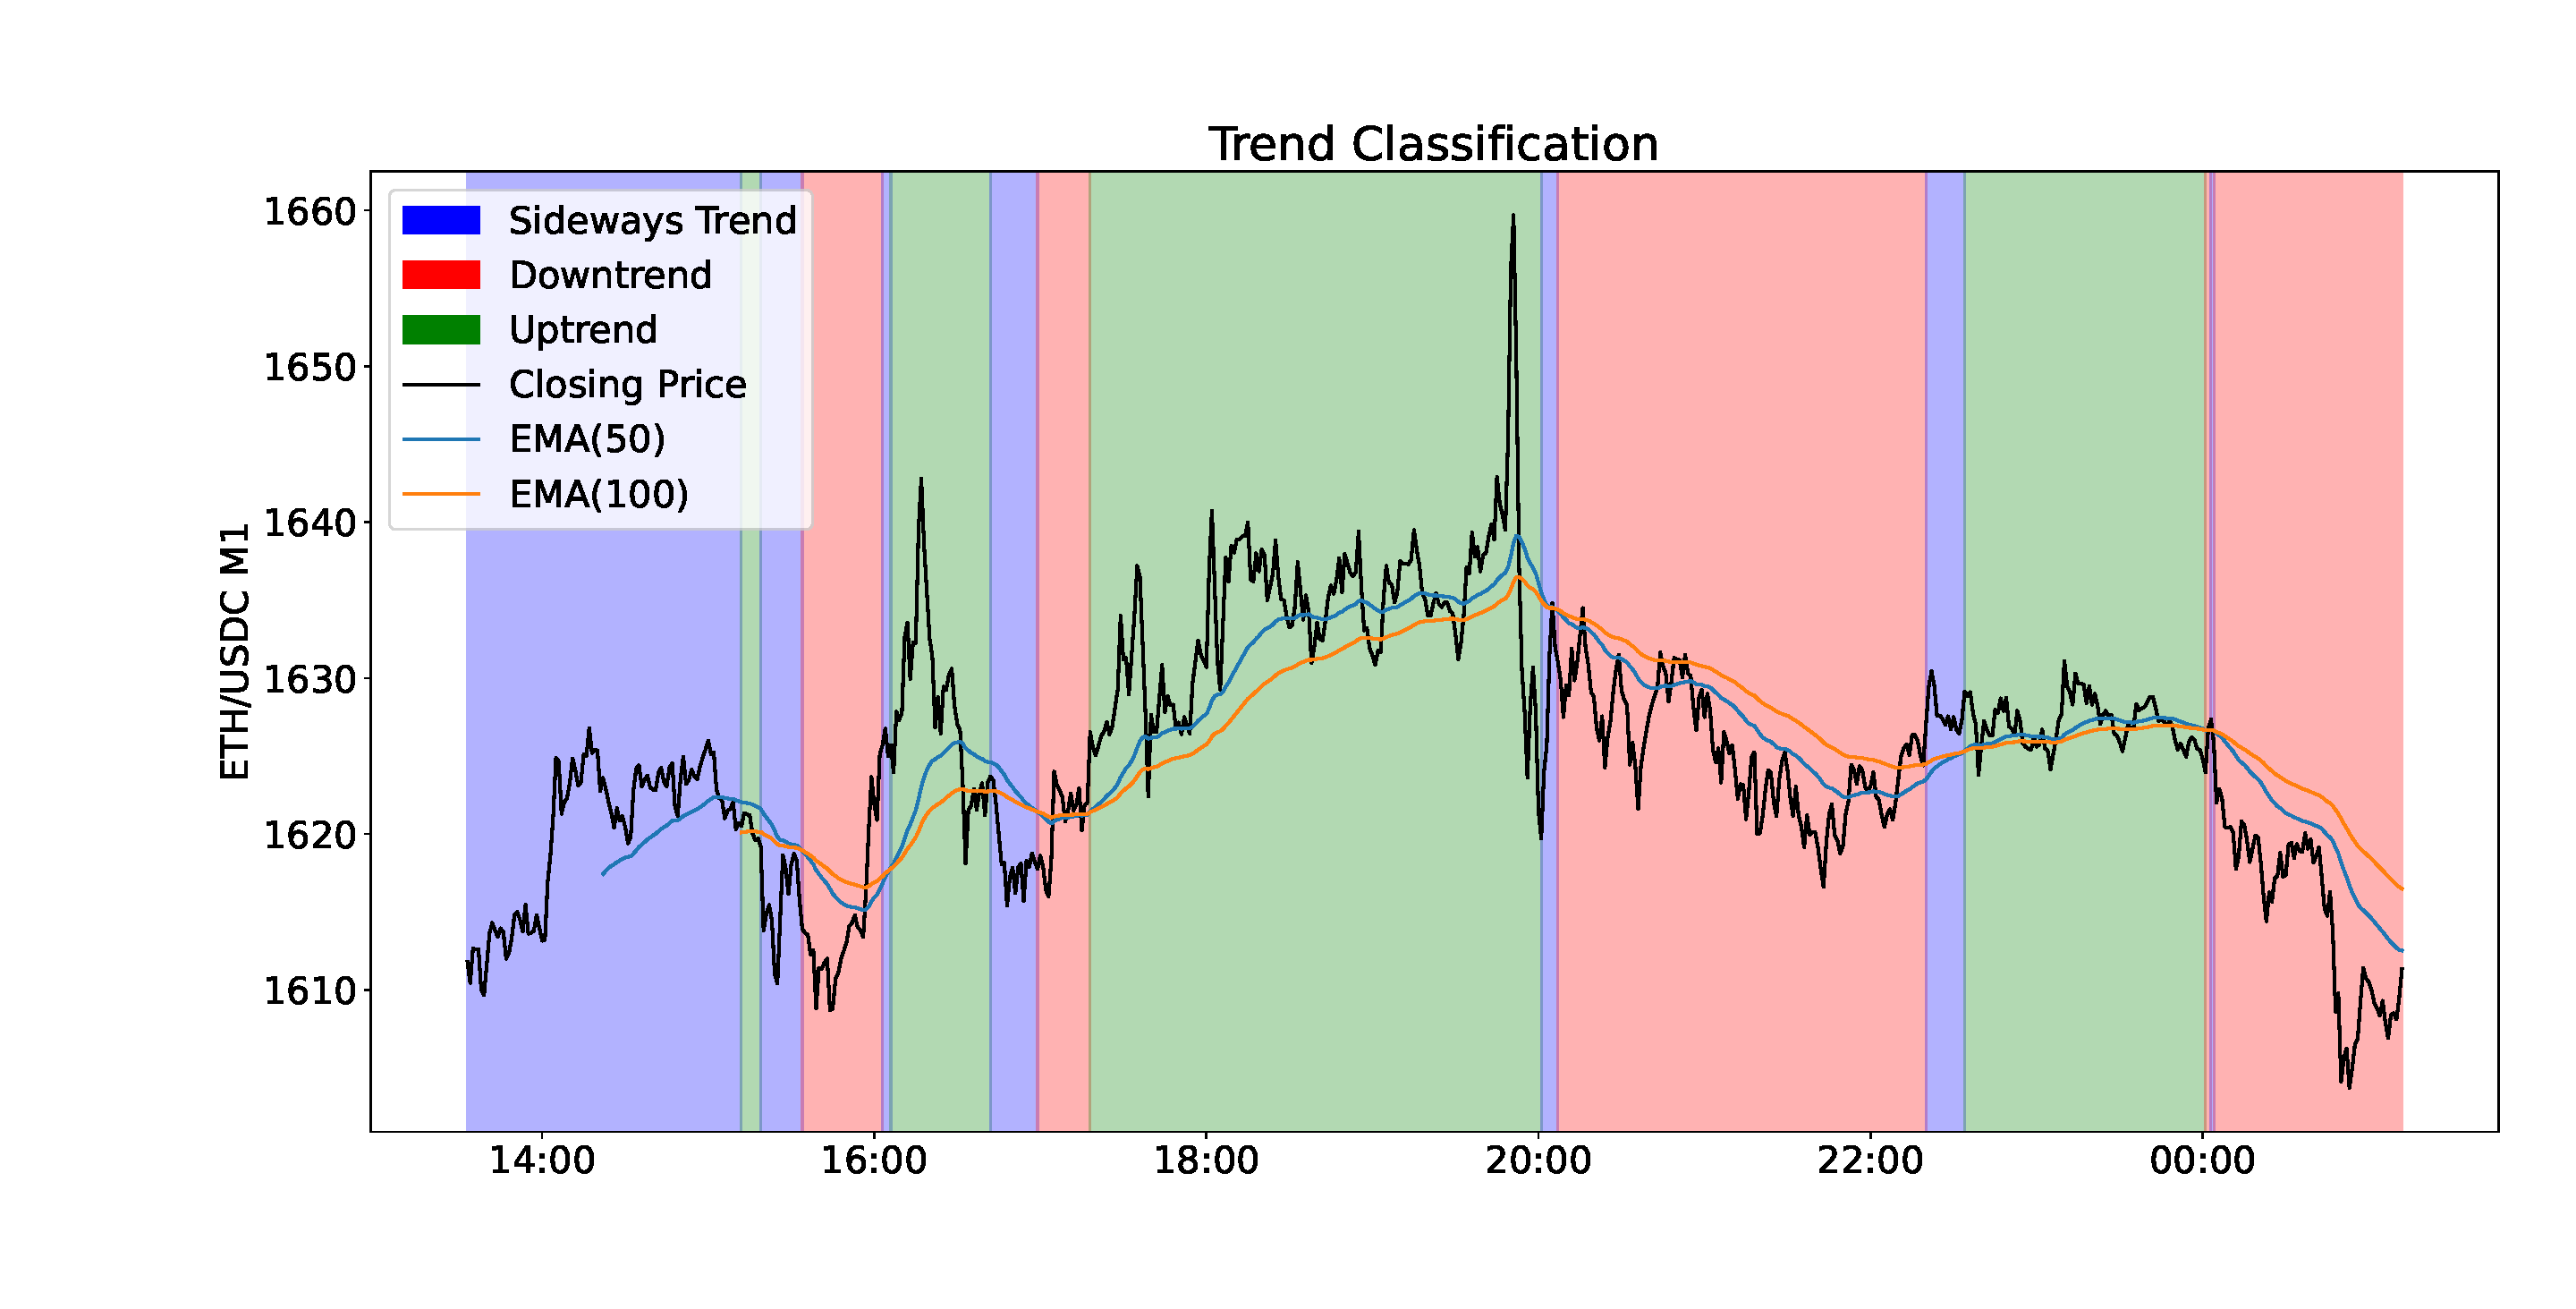
\includegraphics[width=\textwidth]{images/market-regime/market_regime_trend}
    \caption{Trend Classification}
    \label{fig:mr-trend-classification}
\end{figure}

\subsubsection{Recognizing Volatility}
\label{chap:recognizing-vola}

The second step is to categorize the market into phases with high and low volatility.
The volatility is calculated as the standard deviation of the logarithmic returns over the last 30 minutes \cite{wiki-vola}.
This locally calculated volatility depicts short-term fluctuation intensity, and enables a context-dependent assessment of current market behavior.

To classify this local volatility, a comparison is made with the median of all available volatilities in the training dataset which was used for fitting the volatility classification indicator.
If the current volatility is greater than the median, the market is classified as highly volatile.
Otherwise, the market is classified as low volatility.

This threshold definition is deliberately based on a dynamic, data-dependent approach rather than using a fixed absolute threshold.
This automatically adapts the volatility classification to each specific market, and can therefore theoretically be applied to other financial markets.

\autoref{fig:mr-vola-classification} shows the volatility classification on the same base data used in \autoref{fig:mr-trend-classification}.

\begin{figure}[H]
    \centering
    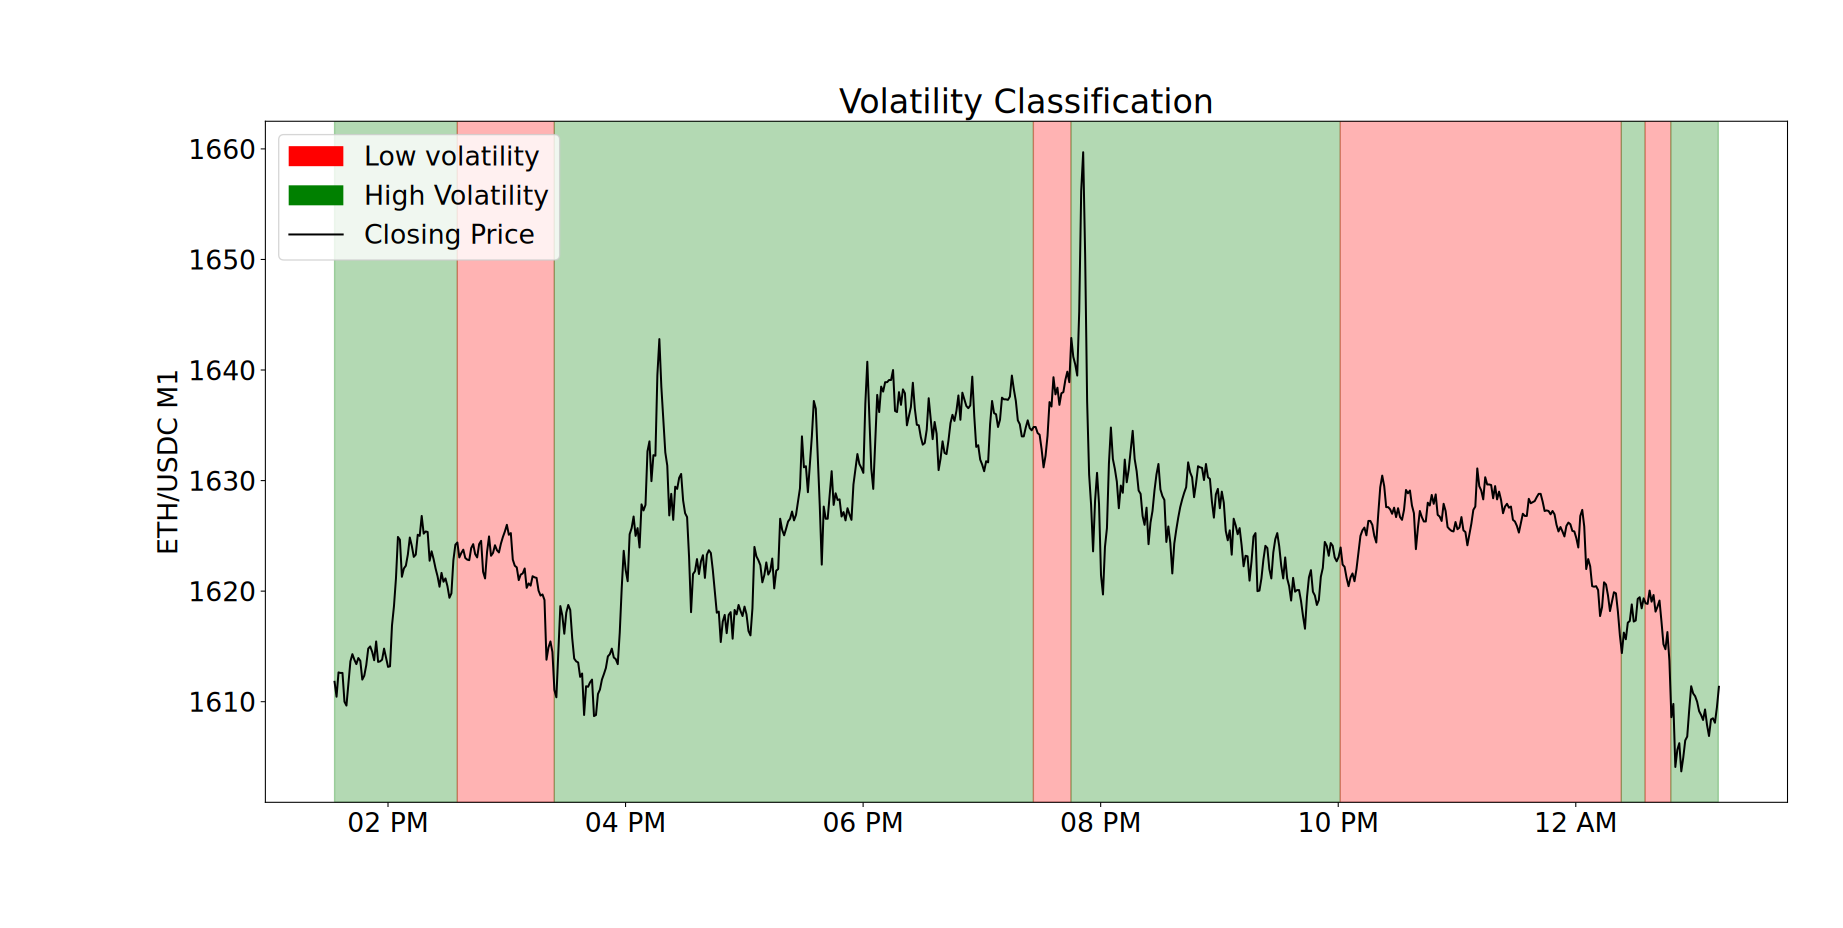
\includegraphics[width=\textwidth]{images/market-regime/market_regime_vola}
    \caption{Volatility Classification}
    \label{fig:mr-vola-classification}
\end{figure}

\subsubsection{Combining Trend and Volatility Classification}

After the two separate classifications in \autoref{chap:recognizing-trend} and \autoref{chap:recognizing-vola} the results can be combined.
The results of the combination can be seen in \autoref{fig:mr-classification}.

\begin{figure}[H]
    \centering
    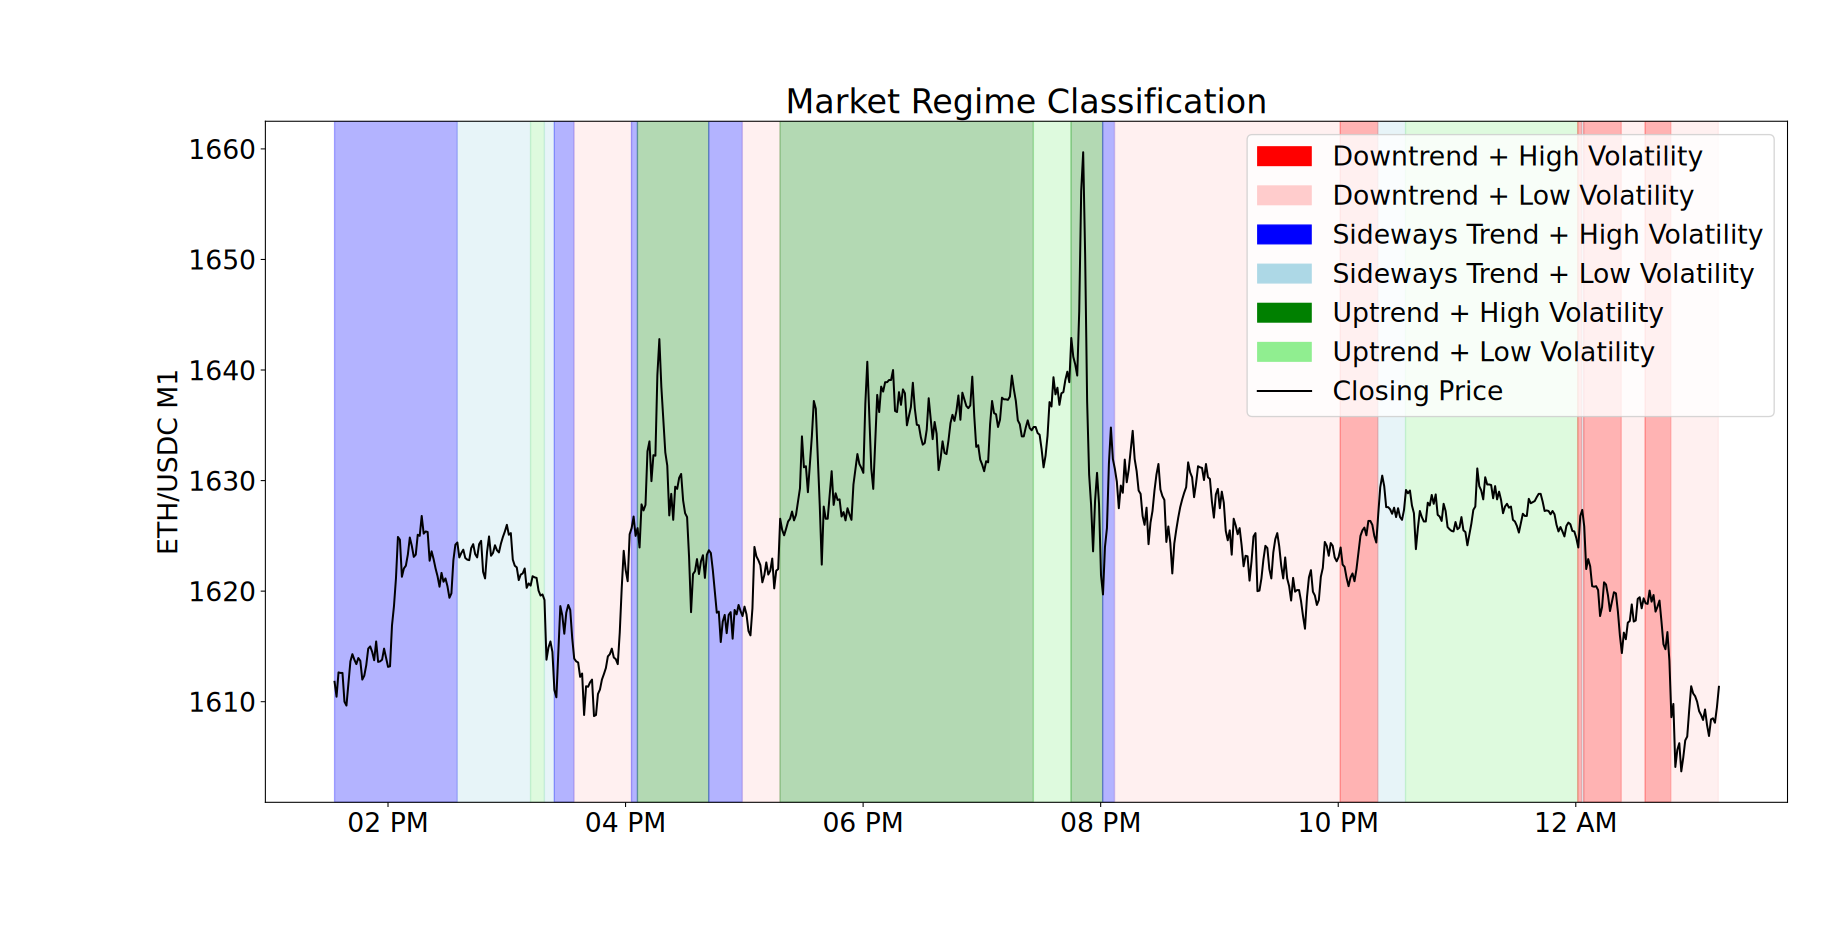
\includegraphics[width=\textwidth]{images/market-regime/market_regime}
    \caption{Regime Classification}
    \label{fig:mr-classification}
\end{figure}

While classification of the market regimes some discrepancies may occur in individual cases between the algorithmically determined category and the visually perceived category.
Such misclassifications are particularly possible during transition phases or in the case of short-term outliers.
For example, the downtrend, highly volatile market regime after 10:00 PM, the algorithm detected a downtrend, but visually, an uptrend is perceived.
At this time, the market is in a transition, which causes this misclassification.

Crucially, the classification distinguishes consistently and meaningfully, which is the case when viewed as a whole.
The robustness and usefulness of the approach does not arise from absolute freedom from errors, but rather from the systematic reduction of uncertainty compared to a purely visual or subjective assessment.

\subsection{Dividing Market Regimes in Durations}

Based on the combination of trend direction and volatility level, the duration of each market regime is also taken into account to enable a more differentiated classification.
The regime duration is divided into three quantiles (33\%, 66\%, 100\%) based on its distribution, allowing for classification into short-term, medium-term, and long-term phases.
The notation in the current work for the respective regime durations is $Q_{0.33}$, $Q_{0.66}$ and $Q_{1}$.

The combination of these three dimensions results in a total of 18 different market regimes.
This fine-grained segmentation makes it possible to more precisely capture and differentiate different market conditions.
For example, a short-term, volatile uptrend from a long-term, calm downtrend.

Even through this makes the market appear more fragmented, and regimes can change more frequently, this finer subdivision is analytically useful.
It allows for context-sensitive market behavior to be examined, and differences in the dynamics of effectiveness of trading strategies in specific regime types to be systematically analyzed.

Instead of smoothing out reality with overly broad categories, a more nuanced picture is deliberately drawn that takes into account both the direction, intensity, and stability of market behavior.
The resulting increased complexity is not a disadvantage, but rather a prerequisite for more meaningful, context-based analyses.



    \newpage

    \section{Money- and Risk-Management}

Successful trading is not only based on a good strategy, but also on a disciplinant management of capital, and risk.
Even the best prediction is useless if losses grow uncontrolled or a majority of the capital is risked by a few wrong decisions.
This is where money, and risk management come into play.
They define clear rules regarding how much to invest per trade, what level of risk is acceptable, and how losses can be limited.
The goal is to protect capital over the long term, minimizing drawdowns, and profit from positive expected values in a controlled manner.
This chapter introduces fundamental concepts, metrics, and methods helping to make rational, and sustainable decisions.

\subsection{Calculating the Position Size}

An important part of risk management is calculating the position size.
It is helpful for maximizing the potential returns, as well as minimizing the financial risk.
Many traders are only willing to risk 1\% or 2\% of the available capital per trade, to prevent a series of losing trades from decimating the available capital too much.

The distance between the estimated entry price, and the estimated stop loss price represents the maximum distance a market can move in an unprofitable direction before a position is automatically closed.

This allows the calculation of the position size to be carried out in three steps:

\begin{enumerate}
    \item \textbf{Determining the risk per trade:} First, it must be determined how much of the available capital should be risked.
    If 1\% of \$10,000 is to be risked, the maximum risk is \$100.
    It is important to note that the fraction of 1\% does not have to be fixed.
    Thus, it is possible to risk more if the entry signal is very clear.
    If the entry signal is less clear, it can also be risked less.
    Only a fixed upper limit should be defined.
    \item \textbf{Calculating the risk per unit:} To calculate the risk per share the absolute distance between the estimated entry price, and the estimated stop loss price must be calculated.
    This represents the risk per unit.
    \item \textbf{Calculate the position size:} Dividing the risked capital by the risk per unit represents the number of units to buy or sell.
\end{enumerate}

In total, these three steps can be combined into one formula \cite{britannica-position-size}:

\begin{equation}
    PositionSize = \frac{Available Balance*RiskPerTrade}{RiskPerUnit}
\end{equation}

So if the available account balance is \$10,000.00, the risk per trade is 1\%, and the distance from the estimated entry price to the stop loss is \$5.
The position size is calculated by:

\begin{equation}
    PositionSize = \frac{\$10.000*1\%}{\$5}=\frac{\$100}{\$5}=20 [Units]
\end{equation}

It is important to note that numbers can result with many decimal places, and many brokers only allow positions with a certain number of decimal places.
If this is the case, the position size must be subsequently rounded to the maximum number of decimal places supported.

\subsection{Validating an Entry Signal}

Not every entry signal generated by a trading strategy is necessarily profitable.
To be profitable in the long term, it is important to ensure that entry signals that are too risky or unrealistic in advance are filtered out, thus preventing positions from being opened.
This chapter presents some techniques that can be used to validate entry signals.

\subsubsection{Risk-Reward-Ratio}

The risk reward ratio (RRR) is a fundamental key figure in trading.
It describes the ratio between the potential profit (reward), and the potential loss (risk) of a single trade.
The RRR helps in deciding wether an entry signal is too risky or not.
It ensures that not only the hit rate determines the success of a strategy, but also the ratio of profit to loss in each individual trade.

The RRR is calculated by:

\begin{equation}
    RRR = \frac{PossibleProfit}{PossibleLoss} = \frac{|OpenPrice - TakeProfitPrice|}{|OpenPrice - StopLossPrice|}
\end{equation}

For example, if a long trade is opened at \$100, with a take profit at \$110, and a stop loss at \$95, the result is:

\begin{equation}
    RRR = \frac{|\$100 - \$110|}{|\$100 - 95\$|} = \frac{\$10}{\$5} = 2
\end{equation}

This means that for every dollar risked, a potential profit of two dollar is targeted.

A RRR greater $1$ is generally considered positive because the expected profit is higher than the potential loss.
However, the RRR should not be viewed in isolation.
The essential factor is the combination of RRR, and hit rate:

\begin{enumerate}
    \item \textbf{High RRR, low hit rate:} e.g.
    $RRR=3$ with only a 30\% probability of winning $\Rightarrow$ potentially profitable.
    \item \textbf{Low RRR, high hit rate:} e.g.
    $RRR=0.5$ with an 80\% hit rate $\Rightarrow$ also potentially profitable.
\end{enumerate}

The following rule of thumb clarifies when a strategy has a positive expected value in the long term:

\begin{equation}
    ExpectedValue = PossibleProfit * HitRatio - PossibleLoss * (1 - HitRatio)
\end{equation}

Only when this expected value is above zero a trading strategy is statistically profitable.

The RRR is not only a mathematical metric, but a central component of risk management.
It helps traders systematically plan how much they are willing to lose per trade, relative to the expected profit.
By consistently applying a minimum RRR (e.g.
$\ge 1.5$), many inefficient setups can be eliminated in advance \cite{bitpanda-crv}.

\subsubsection{Maximum Account Risk}

(Nicht mehr als 10\% des Riskieren in Summe)

\subsubsection{Minimum Take Profit}

In every trading strategy transaction fees play an important role.
Especially in short-term trading transaction fees can turn seemingly profitable trades negative if they are not adequately considered.
A common mistake is setting the take profit level too narrowly, resulting in a profit that is smaller than the costs incurred.
To trade profitably, and sustainably, it is therefore essential that the take profit at least covers the fees incurred, but ideally, significantly higher.

\subsection{Dealing with Trading Fees}
\label{chap:dealing-with-trading-fees}

As shown in \autoref{tbl:broker-comparision} ByBit charges two different fees named maker-, and taker-fee.
The maker fee is charged when a limit order is placed in the order book, thereby creating liquidity.
In contrast, the taker fee is charged when a market order is executed.
This removes liquidity from the market.
It is better for a broker if a market is as liquid as possible.
Therefore, maker orders incur lower fees than taker orders.

Especially in higher-frequency trading, it is better to charge as few fees as possible.
Therefore, it is better for a trader to execute as many limit orders as possible.
Two orders are required for a complete trade: one for entry, and one for exit.
But typically, three orders are placed (entry, stop-loss, take-profit), with either the take-profit or stop-loss order being executed.

If a market order is to be executed as an entry order, it is possible to convert it into a limit order by setting the order price slightly below (for long positions) or slightly above the current price (for short positions).
The same procedure can be followed for the take-profit order.

However, this procedure should not be used for a stop-loss order.
If this is converted to a limit position, there is no longer any guarantee that the stop order will be executed at all, as there is no longer any guarantee that the price will rise above or below the order level.
This means that a position may remain open significantly longer than intended.
If the price then continues to move in an unprofitable direction, the worst-case scenario is that the position is automatically closed by the broker because there is no longer any capital in the account.

The same problem can theoretically occur with a take-profit order.
The difference here, is that the set stop market order still defines the maximum risk.
Thus, while this particular trade may not be profitable, it is impossible to lose all of the capital.
It is similar with the opening order.
If it is not executed, the entire trade is not going to be executed.
This means a missed potential profit, but there is no risk of losing capital.

If all orders are executed as planned, and the price moves in a profitable direction, the conversion of the orders will result in a reduction of fees by a factor of 2.75.

    \newpage

    \section{Deep Learning Models}
\label{chap:dl-models}

This chapter presents the key components for developing and evaluating deep learning models.
This includes both the selection of suitable models and the criteria for assessing their performance.

For this work, Keras version 3.10.0 was used as a high-level API for modeling and training neural networks \cite{keras-home}.
Instead of the standard TensorFlow backend, PyTorch version 2.7.1 was used as the backend.
A key reason for this decision was its better support on Windows, compared to TensorFlow \cite{tf-windows}, particularly with regard to installation and compatibility with existing CUDA drivers.
By using Keras in combination with the PyTorch backend, user-friendly modeling could be combined with stable and well-supported execution on Windows systems.

%TODO: Es werden Regressions und Klassifikationsmodelle trainiert

The model architectures used in this work are not based on specific, citable publications, but were designed as part of an experimental and iterative development process.
The goal was to construct powerful models well-suited to the given problem.
Particularly with regard to processing sequential data of limited length and high variability.

Established neural building blocks such as 1D convolutional layers, GRUs, attention mechanisms, and transformer components were used, the fundamentals of which are comprehensively documented in the literature.
However, the specific design of the model architectures, such as the combination of multiple parallel CNN paths, the integration of GRUs after convolution steps, or the use of Global Average Pooling instead of flattening, represents a creative and pragmatic composition of its own.

Additionally, all models were automatedly optimized using Optuna, so that architectural decisions were also influenced by the hyperparameter search.
In many cases, initial ideas originate from non-scientific sources such as blog posts, online tutorials, or community code snippets, which are not scientifically citable.

In summary, the developed models are original variations, inspired by familiar architectural elements, but not directly adopted or reconstructed from specific publications.
This allows for greater flexibility and reinforces the experimental nature of the work.

For both regression and classification models, 13 different architectures were used, which can be divided into neural networks, convolutional neural networks, long short-term memories, and transformers.

\subsection{Metrics}

% TODO

\subsection{Optuna}

In modern machine learning methods, the selection of hyperparameters plays a central role in model performance.
Hyperparameters such as learning rate, the number of layers in a neural network, or regularization strengths directly influence the behavior and generalization of the model.
The search for optimal values for these parameters, the so-called hyperparameter optimization, is often a time-consuming and computationally intensive process \cite{hyperparameter-importance}.

Optuna is a modern framework for automated hyperparameter optimization designed for efficiency, flexibility, and ease of use.
It was developed to enable easy integration into existing machine learning pipelines while providing powerful, goal-oriented optimization.

The goal of Optuna is to automatically find those hyperparameter combinations that satisfy a specific optimization criterion (e.g., minimum validation error rate or maximum accuracy).
The search process should be as efficient as possible, requiring as few model training sessions as possible \cite{optuna-hyperparameters}.

In this work, Optuna was used to automatically run multiple training models with different hyperparameters to find the best hyperparameters.
In the relevant sections of the next chapters, the range of the hyperparameters for each model will be mentioned.

\subsection{Neural Networks}
\label{chap:nn}

Neural networks are among the central methods of machine learning and form the basis of many modern deep learning models.
The simplest and most widely used form is the feedforward neural network (FNN), also known as a multilayer perceptron (MLP).
Such networks are universally applicable and, with appropriate structuring, can be used for classification, regression, and pattern recognition.

A classic neural network consists of several layers of artificial neurons that forward information in a fixed order from input to output.
The structure can be divided as follows \cite{nn-basics}:

\begin{enumerate}
    \item \textbf{Input Layer:} Accepts the raw input data, e.g., a vector form of a time series or preprocessed features.
    \item \textbf{Hidden Layers:} One or more layers of artificial neurons, each of which calculates a weighted sum of the inputs and further processes it using an activation function.
    Typical activation functions are ReLU, sigmoid, or tanh.
    \item \textbf{Output Layer:} Provides the final result, e.g., class membership (for classification) or continuous value (for regression).
\end{enumerate}

In this work, three different neural network models have been tested.
The tested models are different in their complexity, depth, and methodical approach to data processing.

\subsubsection{Base Model with Flatten-Architecture}

The first model follows a classic feedforward approach, with one to three dense layers, each with 32 to 128 neurons and a rectified linear unit (ReLU) activation function.
The ReLU activation function was used because it provides an efficient calculation and a good gradient propagation with fewer vanishing gradients \cite{springer-ml-basics}.
Either before or after the dense layers, the input data are flattened \cite{keras-flatten}.
This decision influences whether the model processes all timepoints as a vector early on or treats each time step separately.
This architecture was used as a simple baseline model to obtain a quick training and a first baseline model.

The learning rate of the Adam optimizer ranges between $10^{-5}$ and $10^{-2}$, while the input layer has a length of 5 to 150
All hyperparameters are managed by Optuna.

\lstinputlisting[language=Python, caption=Base FNN, label=lst:base-model, style=python]{python/models/nn_base.py}

\subsubsection{Dropout Neural Network}

In the second model, the data is first converted into a one-dimensional vector using a flatten layer.
This is followed by one to three dense layers using ReLu activation.
Batch normalization supports stable and rapid convergence \cite{batch-normalization}, while dropout between 5\% and 35\% of the data is used as a regularization method to prevent overfitting \cite{keras-dropout}.
All other parameters are identical to those in the simple neural network.

The parameters tuned via Optuna control the model depth, the number of nodes per layer, the training dynamics, and the number of historical time points used as input.

\lstinputlisting[language=Python, caption=Dropout NN, label=lst:dropout-nn, style=python]{python/models/nn_dropout.py}

\subsubsection{Residual Neural Network}

The third model integrates a residual concept, originally known from image processing but also increasingly used in time series contexts.
The architecture consists of a linear shortcut branch connected to the main path via an additive connection \cite{residual-nn}.
This construction facilitates the training of deeper networks by improving gradient flow and preventing information loss through multiple layers.

In addition to the previous parameters, two additional variables controlled by Optuna are added: \verb|num_units_res_prep| and \verb|num_units_res|.
These determine the complexity of the residual branch.
The distinction whether flattening is done before or after the hidden layers is also included here to flexibly adapt data processing to the underlying data structure.

This architecture is particularly suitable for nonlinear and complex relationships, such as those frequently encountered in ETH price forecasting.
The residual path allows the model to pass on basic information directly, while deeper layers learn abstract features.

\lstinputlisting[language=Python, caption=Residual NN, label=lst:residual-nn, style=python]{python/models/nn_residual.py}

\subsection{Long Short-Term Memory Models}
\label{chap:lstm}

In addition to traditional dense neural networks, recurrent neural networks (RNNs) based on the Long Short-Term Memory (LSTM) architecture were also used.
LSTMs are specifically designed to capture temporal dependencies in sequential data and retain long-term information across multiple time steps \cite{lstm-usage}.
This is particularly important for financial data such as ETH prices, as current prices are often influenced by past developments.

LSTM cells have an internal memory structure and three control mechanisms (input, forget, and output gates) that allow the network to decide which information should be stored, overwritten, or passed on \cite{lstm-cell}.
This effectively mitigates the so-called vanishing gradient problem of traditional RNNs \cite{lstm-gradient-problem}.

\subsubsection{Base LSTM}

This model consists of one or two stacked LSTM layers followed by a dense output layer.
If only one LSTM layer is added, it returns the result directly.
With multiple layers, the temporal sequence information is passed to the second LSTM layer.

Similar to feedforward neural networks, the number of layers, the number of neurons per layer, the learning rate, and the length of the input window used are managed via Optuna.

This model represents the basic form of a sequential predictor and is well suited for simple time series patterns.

\lstinputlisting[language=Python, caption=Base LSTM, label=lst:base-lstm, style=python]{python/models/lstm.py}

\subsubsection{Dropout LSTM}

This variant extends the standard model with dropout layers inserted between the LSTM units, discarding between 5\% and 50\% of the data.

The additional parameter is also determined by Optuna and allows fine-tuned control over the regularization strength.
This model is particularly useful when working with noisy or volatile price trends, such as cryptocurrencies.

\lstinputlisting[language=Python, caption=Dropout LSTM, label=lst:dropout-lstm, style=python]{python/models/lstm_dropout.py}

\subsubsection{Bidirectional LSTM (BiLSTM)}

The third model uses bidirectional LSTM layers.
These process the input sequence forward and backward simultaneously, allowing both earlier and later information to be incorporated into the internal state \cite{bi-lstm}.

This architecture can be particularly valuable in the context of ETH predictions based on historical data, as it allows for better detection of symmetric patterns or turning points in price trends.

The hyperparameter structure is similar to the previous models, but the modeling is performed using double LSTM paths.

\lstinputlisting[language=Python, caption=Bidirectional LSTM, label=lst:bi-lstm, style=python]{python/models/lstm_bi.py}

\subsubsection{Encode-Decode Model with Repeat-Vector}

The fourth model is based on an encoder-decoder approach, as used in machine translation.
The input sequence is first converted into a fixed context vector by an LSTM layer, which is then duplicated multiple times using RepeatVector \cite{keras-repeat-vector}.
A decoder-LSTM interprets this vector sequentially to generate a temporally structured output.

This architecture is particularly suitable for multistep forecasting, as it can map not only the next value but an entire sequence of future values.
The final preprocessing is performed using \verb|TimeDistributed(Dense(...))| to calculate a separate output for each time step \cite{keras-time-distributed}.

\lstinputlisting[language=Python, caption=Encode-Decode LSTM, label=lst:encode-decode-lstm, style=python]{python/models/lstm_encode_decode.py}

\subsection{Convolutional Neural Networks}
\label{chap:cnn}

Convolutional neural networks (CNNs) represent a special architecture within deep learning that was developed specifically to process data with spatial structures, such as images.
Compared to traditional feedforward networks, CNNs are significantly more efficient in handling high-dimensional inputs and have established themselves as standard methods in numerous application areas such as object detection, natural language processing, and time series analysis \cite{cnn-for-time-series}.

The key difference between CNNs and classical neural networks lies in the use of so-called convolutional layers, which exploit the local structures in the input data.
Instead of connecting every neuron to all input values (as with a fully connected layer), local filters (kernels) are used that respond only to a small portion of the input space.
These filters are automatically learned during the training process \cite{cnn-for-time-series}.

Time series typically exhibit temporal dependencies, repetitions, seasonal patterns, or short-term fluctuations.
Classic methods for processing this data, such as LSTM networks, explicitly model such dependencies using recursive states.
CNNs, on the other hand, uses an alternative approach, called local convolutions, which also serve time series to detect relevant patterns or changes over short or medium periods of time \cite{cnn-local-convolution}.

The advantages of using CNNs for time series include:

\begin{enumerate}
    \item \textbf{Parallel Processing:} CNN does not require recursive loops, e.g., compared to LSTMs.
    \item \textbf{Local Pattern Detection:} CNNs can detect local patterns, such as peaks, fluctuations, or trend changes.
    \item \textbf{Computational Complexity:} CNNs requires lower computational power compared to recursive architectures.
\end{enumerate}

\subsubsection{Base CNN}

The simplest variant consists of two stacked one-dimensional convolutional layers, followed by maxpooling, and two dense layers for output preparation.
The position of the flattening layer affects the processing order between the dense and the sequence structure.

The hyperparameters tuned by Optuna are the number of units in the convolutional layers, the length of the filters (Kernel size), the size of the maxpooling region, the position of the flattening layer, and the number of neurons in the dense layers.

\lstinputlisting[language=Python, caption=Base CNN, label=lst:simple-cnn, style=python]{python/models/cnn_simple.py}

\subsubsection{Deep CNN}

The model shown here represents an extension of a simple CNN model (Base CNN).
While the simple model uses only a single 1D convolutional layer followed by a pooling and dense layer, this Deep CNN model uses two consecutive Conv1D layers.
This additional depth allows the network to learn more complex and hierarchical feature representations from the input data \cite{cnn-deep-more-complex}.
This is particularly useful for timeseries with multi-level dependencies or subtle patterns.
The model is complemented by a MaxPooling layer, which reduces the temporal resolution and counteracts overfitting.
The optional placement of the Flatten layer allows for the evaluation of different configurations of feature identification, which in turn increases model flexibility.
Overall, this more deeply structured CNN enables more powerful modeling than the flattened variant.

\lstinputlisting[language=Python, caption=Deep CNN, label=lst:deep-cnn, style=python]{python/models/cnn_deep.py}

\subsubsection{Attention CNN}

An alternative architecture uses multiple parallel convolutional layers with different kernel sizes.
This allows the model to detect both short-term and medium-term patterns simultaneously.
The resulting feature maps are combined using an attention layer to highlight important sequence segments \cite{cnn-attention}.

This is followed by global average pooling and a dense layer for output generation.

\lstinputlisting[language=Python, caption=Attention CNN, label=lst:attention-cnn, style=python]{python/models/cnn_attention.py}

\subsubsection{Concatenation CNN}

A slightly modified version replaces the attention module with a simple concatenation of the feature maps.
This allows the model to pass the extracted features directly without performing weighting \cite{keras-concat}.

This variant is computationally less expensive than the attention-based one and is well-suited when all filter outputs should be treated equally.

\lstinputlisting[language=Python, caption=Concatenation CNN, label=lst:multiscale-cnn, style=python]{python/models/cnn_multi_scale.py}

\subsubsection{CNN-GRU Hybrid Model}

The Gated Recurrent Unit (GRU) model is a simplified variant of the LSTM and was developed to reduce computational effort and model complexity.
Compared to LSTM, GRU has only two gates, an update gate and a reset gate, instead of three (input, forget, and output gates in LSTM).
This makes GRU faster to train, requires less memory, and delivers comparable results in many tasks \cite{gru-basics}.

To combine the advantages of both architectures, a hybrid CNN-GRU model was also implemented.
A Conv1D layer first extracts local features from the sequence, which are then sequentially processed using a GRU module to capture long-term dependencies and trends \cite{cnn-gru}.

This model is particularly well-suited for linking local patterns (using CNN) with temporal dependencies (using GRU).
The final dense layers perform the transformation to the target variable as usual.

\lstinputlisting[language=Python, caption=CNN + GRU, label=lst:gru-cnn, style=python]{python/models/cnn_gru.py}

\subsection{Regression Models}
\label{chap:regression-models}

Regression models were used to predict the next 30 minutes of logarithmic returns as a continuous sequence.
For this purpose, all models mentioned in \autoref{chap:nn}, \autoref{chap:lstm}, and \autoref{chap:cnn} were trained on the training data (\autoref{tbl:train-data}) for 20 trials of Optuna with 30 epochs each.
After each epoch, the model was evaluated using the validation data (\autoref{tbl:validation-data}).
To achieve a continuous sequence as output, the activation function in the last dense layer of the above-mentioned models was set to \verb|linear| and the number of neurons to 30.

\subsubsection{Loss-Function}
\label{chap:regression-loss}

In order to incorporate the trading context during model training and evaluation, traditional loss functions such as the root mean squared error have been avoided.
Instead, a proprietary loss function was implemented that calculates realized profit and loss.
The value of the loss function decreases the more profit is generated.

As mentioned above, the output of the regression models are either a sequence of the next expected logarithmic returns by minute.
The first step of the loss function is to decide whether the opened position should be a long or short position.
This is decided by cumulating the predictions.
The absolute maximum is then determined for the cumulative values greater than and less than zero.
If the absolute maximum of the values greater than zero is greater than the absolute maximum of the values less than zero, a long position is opened.
Otherwise, a short position is opened.
\autoref{fig:loss-long-position-decision} illustrates the decision using a long position as an example.

\begin{figure}[H]
    \centering
    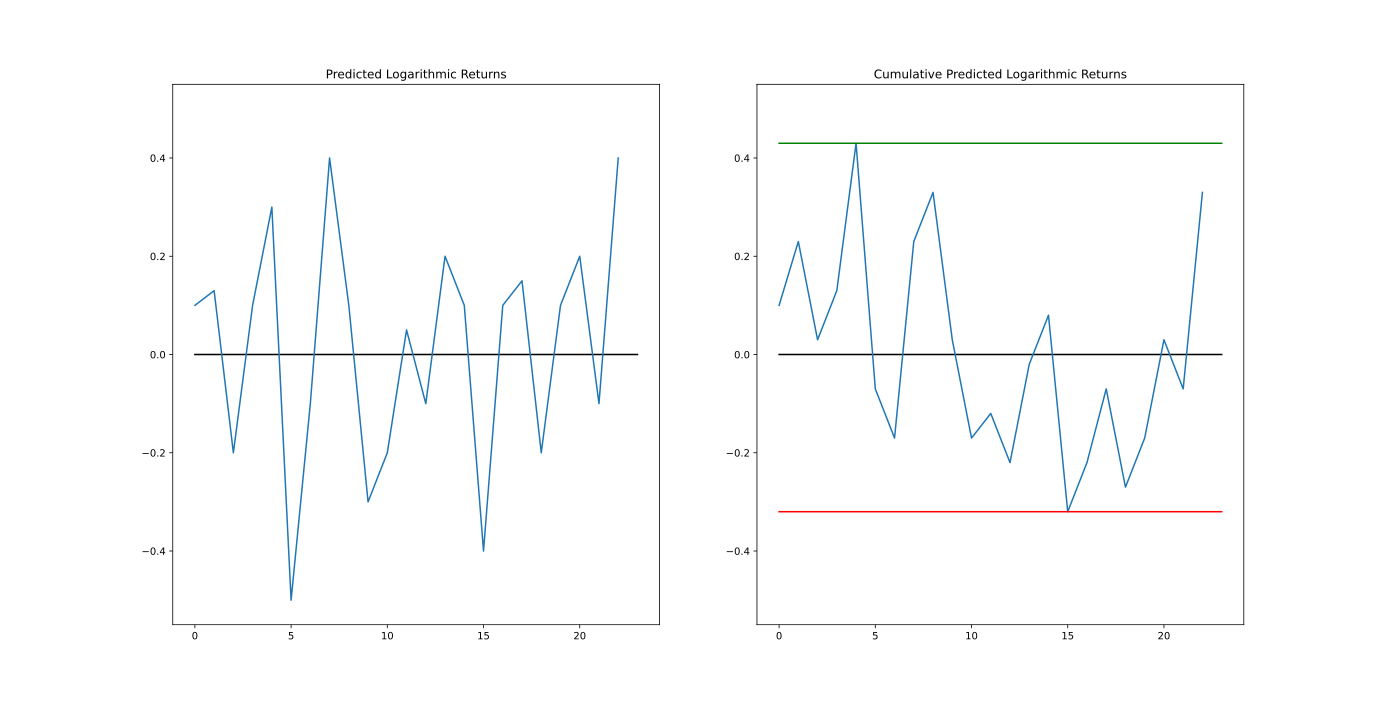
\includegraphics[width=\textwidth]{images/models/loss_direction}
    \caption{Long Position Decision}
    \label{fig:loss-long-position-decision}
\end{figure}

After the direction decision, the stop-loss and take-profit levels must be determined.
For long and short positions, there are two possibilities at which specific level the stop-loss and take-profit are set, based on the global high and low of the cumulative predicted logarithmic returns.
If a long position was previously decided and the global high comes after the global low, the stop-loss is set at the global low and the take-profit at the global high.
However, if the global high comes before the global low, the stop-loss is set at the lowest low before the global high.
For short positions, the decision is exactly the opposite.

\autoref{fig:loss-tp-sl} shows the stop-loss and take-profit levels for all four cases.
The red areas mark the predicted unprofitable zones and the green areas mark the predicted profitable zones.

\begin{figure}[H]
    \centering
    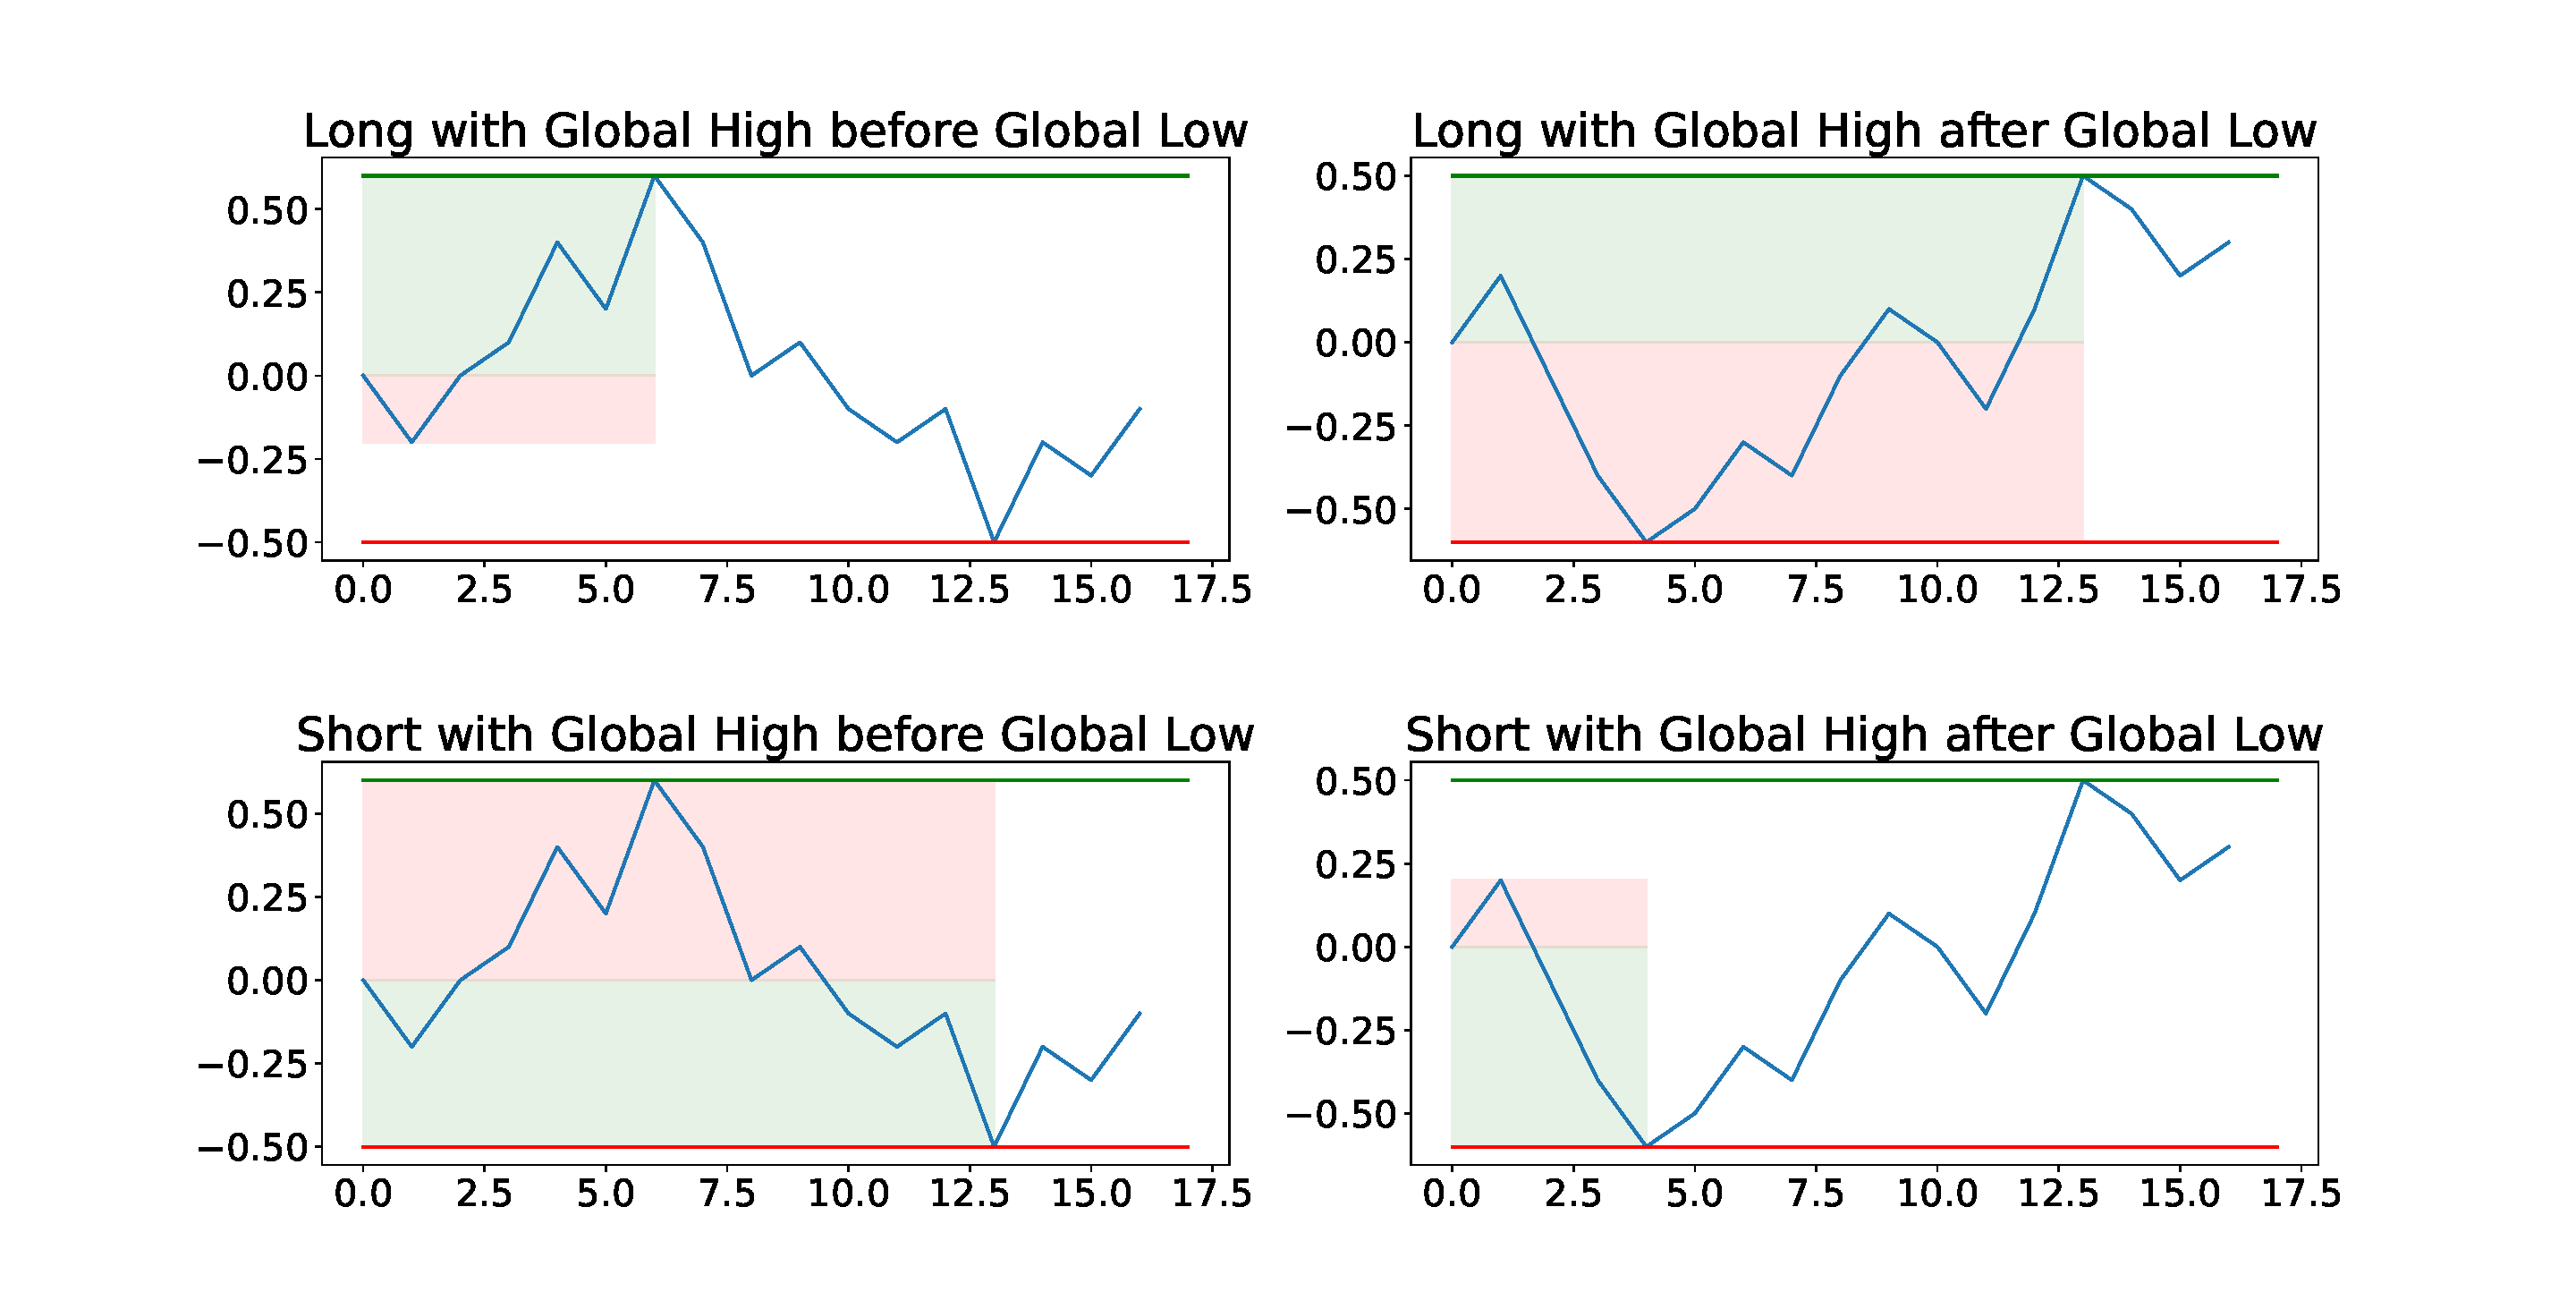
\includegraphics[width=\textwidth]{images/models/loss_tp_sl}
    \caption{Long Position Decision}
    \label{fig:loss-tp-sl}
\end{figure}

After the stop-loss and take-profit levels are determined, the actual logarithmic returns are used to calculate the profit or loss for each position.
If neither the stop-loss nor the take-profit is reached, the profit calculation defaults to the profit if the stop-loss is reached to ensure that the model predicts the correct take-profit more often.

\subsubsection{Model Evaluation}

%TODO

\subsection{Classification-Models}
\label{chap:classification-models}

Classification models were used to predict an action to be performed.
The action can be either buy, sell, or do nothing.
For that, the model predicts a probability for each of the three classes.
As with the \hyperref[chap:regression-models]{regression models}, the same models are used, but this time the last dense layer has only three neurons and the activation function \verb|softmax|.
The identical training and validation period was also used, and the training took place over 20 Optuna trials with 30 epochs each.

\subsubsection{Loss-Function}

For classification models, the categorical cross-entropy loss function was used.
This choice is common and well-suited for classification problems where the model output represents a probability distribution across multiple classes.
Mathematically, it is defined as follows:

\[
    L_{CCE} = -\sum_{i=1}^{C} y_i*log(\hat{y_i})
\]

Where $C$ denotes the number of classes, $y_i$ the actual value (usually encoded as a one-hot vector), and $\hat{y_i}$ the probability predicted by the model for class $i$.
This function penalizes the model particularly severely if it assigns a high probability to an incorrect class and rewards correct predictions with high confidence.

Categorical cross-entropy measures the difference between the actual target distribution and the probability distribution predicted by the model \cite{springer-ml-basics}.

\subsubsection{Model Evaluation}

%TODO

    \newpage

    \usepackage{hyperref}


\section{Trading Strategies}
\label{chap:trading-strategies}

In the context of automated trading, systematic trading strategies play a central role.
They enable decisions to be made based on clearly defined rules or mathematical models, rather than on subjective assessments or human intuition.

A trading strategy defines a methodical approach by which financial instruments are bought or sold to achieve a specific goal.
Typically, this is to maximize profit while limiting risk.
Such strategies are often based on indicators from technical analysis or fundamental market information \cite{investopia-trading-strategy}.

Essential components of a strategy are signal generation (entry/exit criteria), risk management (e.g., stop-loss, position sizes), and performance evaluation based on metrics such as cumulative profit, volatility, or maximum drawdown.
The development process of a successful strategy typically comprises several phases, ranging from idea generation and backtesting to optimization and validation on previously unseen market data \cite{investopia-trading-strategy-components}.

Similar to deep learning hyperparameters, trading strategies have also parameters, which can be defined before executing.
In this work, these parameters are defined in a range, consisting of a minimal value, a maximum value, and a step size.

This chapter provides an overview of the trading strategies compared in this paper.
Both the models trained in \autoref{chap:dl-models} and classic trading strategies are presented.
An overview of the metrics used to compare the trading strategies is also provided.
The presented strategies also have their parameters defined, which will be tested later.
It should be noted that each strategy also contains a parameter that defines whether positions are opened with a fixed stop level or a trailing stop.
Since this parameter is included in all strategies, it is not listed every time.

\subsection{AI Trading Strategies}
\label{chap:ai-strategies}

AI trading strategies treat the model outputs differently.
Here, too, a distinction is made between regression and classification models.

\subsubsection{Regression AI Strategy}
\label{chap:regression-ai-stategy}

As described in \autoref{chap:regression-models-evaluation}, the trained regression models are not suitable for developing a trading strategy.
Nevertheless, this chapter describes a trading strategy that could be implemented using a predicted series of logarithmic returns.
However, it is not evaluated or tested.

From the predicted series of logarithmic returns, the expected price in $t$ minutes can be calculated by the formula mentioned in \autoref{chap:log-returns}.

Based on the predicted price, the stop-loss and take-profit can be determined identically to the loss-function of the regression models (\autoref{chap:regression-loss}).
This creates an entry signal with fixed stop-loss and take-profit level.

However, since it is possible that the price could exceed the stop level or the take-profit level might not be reached, additional parameters are introduced into the strategy that shift the two levels by a specific number of points.
A third parameter is also introduced, which specifies a fixed distance to the stop-loss if no stop-loss has been predicted.
This can happen, for example, if the initial prediction is positive and the price in the prediction does not fall below the current price.

\begin{table}[H]
    \centering
    \begin{tabular}{L{4cm}ccc}
        \toprule
        \textbf{Parameter Name} & Min Value & Max Value & Step Size
        \\
        \midrule
        \textbf{Take-Profit Delta}             & -20.0 & 20.0 & 2.0  \\
        \textbf{Stop-Loss Delta}               & -20.0 & 20.0 & 2.0  \\
        \textbf{Stop-Loss not Predicted Delta} & 1.0   & 20.0 & 20.0 \\
        \bottomrule
    \end{tabular}
    \caption{AI Regression Model Strategy Parameters}
    \label{tbl:regression-strategy-parameters}
\end{table}

\subsubsection{Classification AI Strategy}

As described in \autoref{chap:classification-models} the classification models predict a probability for an action, which can be either buy, sell or do nothing.
This strategy executes a buy or sell action if the predicted probability is greater than a predefined minimum probability.
If the buy or sell probability is less than the minimum probability or the do nothing probability is the greatest, the strategy does nothing.

The stop-loss and take-profit levels are also predefined parameters.

\begin{table}[H]
    \centering
    \begin{tabular}{L{4cm}ccc}
        \toprule
        \textbf{Parameter Name} & Min Value & Max Value & Step Size
        \\
        \midrule
        \textbf{Take-Profit Distance}       & 5.0 & 100.0 & 5.0 \\
        \textbf{Stop-Loss Distance}         & 5.0 & 100.0 & 5.0 \\
        \textbf{Min. Probability for Entry} & 0.3 & 0.9   & 0.1 \\
        \bottomrule
    \end{tabular}
    \caption{AI Classification Model Strategy Parameters}
    \label{tbl:classification-strategy-parameters}
\end{table}

\subsection{Classic Trading Strategies}

Technical analysis (TA) is based on the assumption that market movements do not develop randomly, but follow certain patterns that have repeated themselves in the past.
In contrast to fundamental analysis, which deals with the intrinsic value of a financial instrument, technical analysis focuses exclusively on past price and volume movements to draw conclusions about future price developments.

Technical analysis focuses on visual and computational methods for identifying trend, support and resistence levels, and reversal points.
These analysis are used to develop specific trading strategies that specifically respond to specific market behaviours.
These strategies are often rule-based and can be implemented both manually and algorithmically \cite{ta-basics}.
Therefore, technical analysis strategies are more likely suitable for algorithmic trading.

This chapter describes three widely used technical analysis trading strategies.
The strategies introduced are not the only classic strategies tested.
They are the three that performed best in the tests.
The other tested strategies are also briefly listed in C\autoref{chap:other-strategies-results}. %TODO: verlinkung
However, some of them have been slightly modified in this work compared to the most widely used ones.

\subsubsection{Dual Simple Moving Average Strategy}
\label{chap:sma2}

A common trading strategy is the simple moving average crossover strategy.
It consists of two SMA with different periods.
If the short-term SMA crosses the long-term SMA above, a long position is opened.
Otherwise, if the short-term SMA crosses the long-term SMA below, a short position is opened \cite{sma-strategy-basics}.
\autoref{fig:sma-example} shows exemplary two moving averages for a synthetic price, with blue arrows marking buy entry signals and red arrows marking sell entry signals.

\begin{figure}[H]
    \centering
    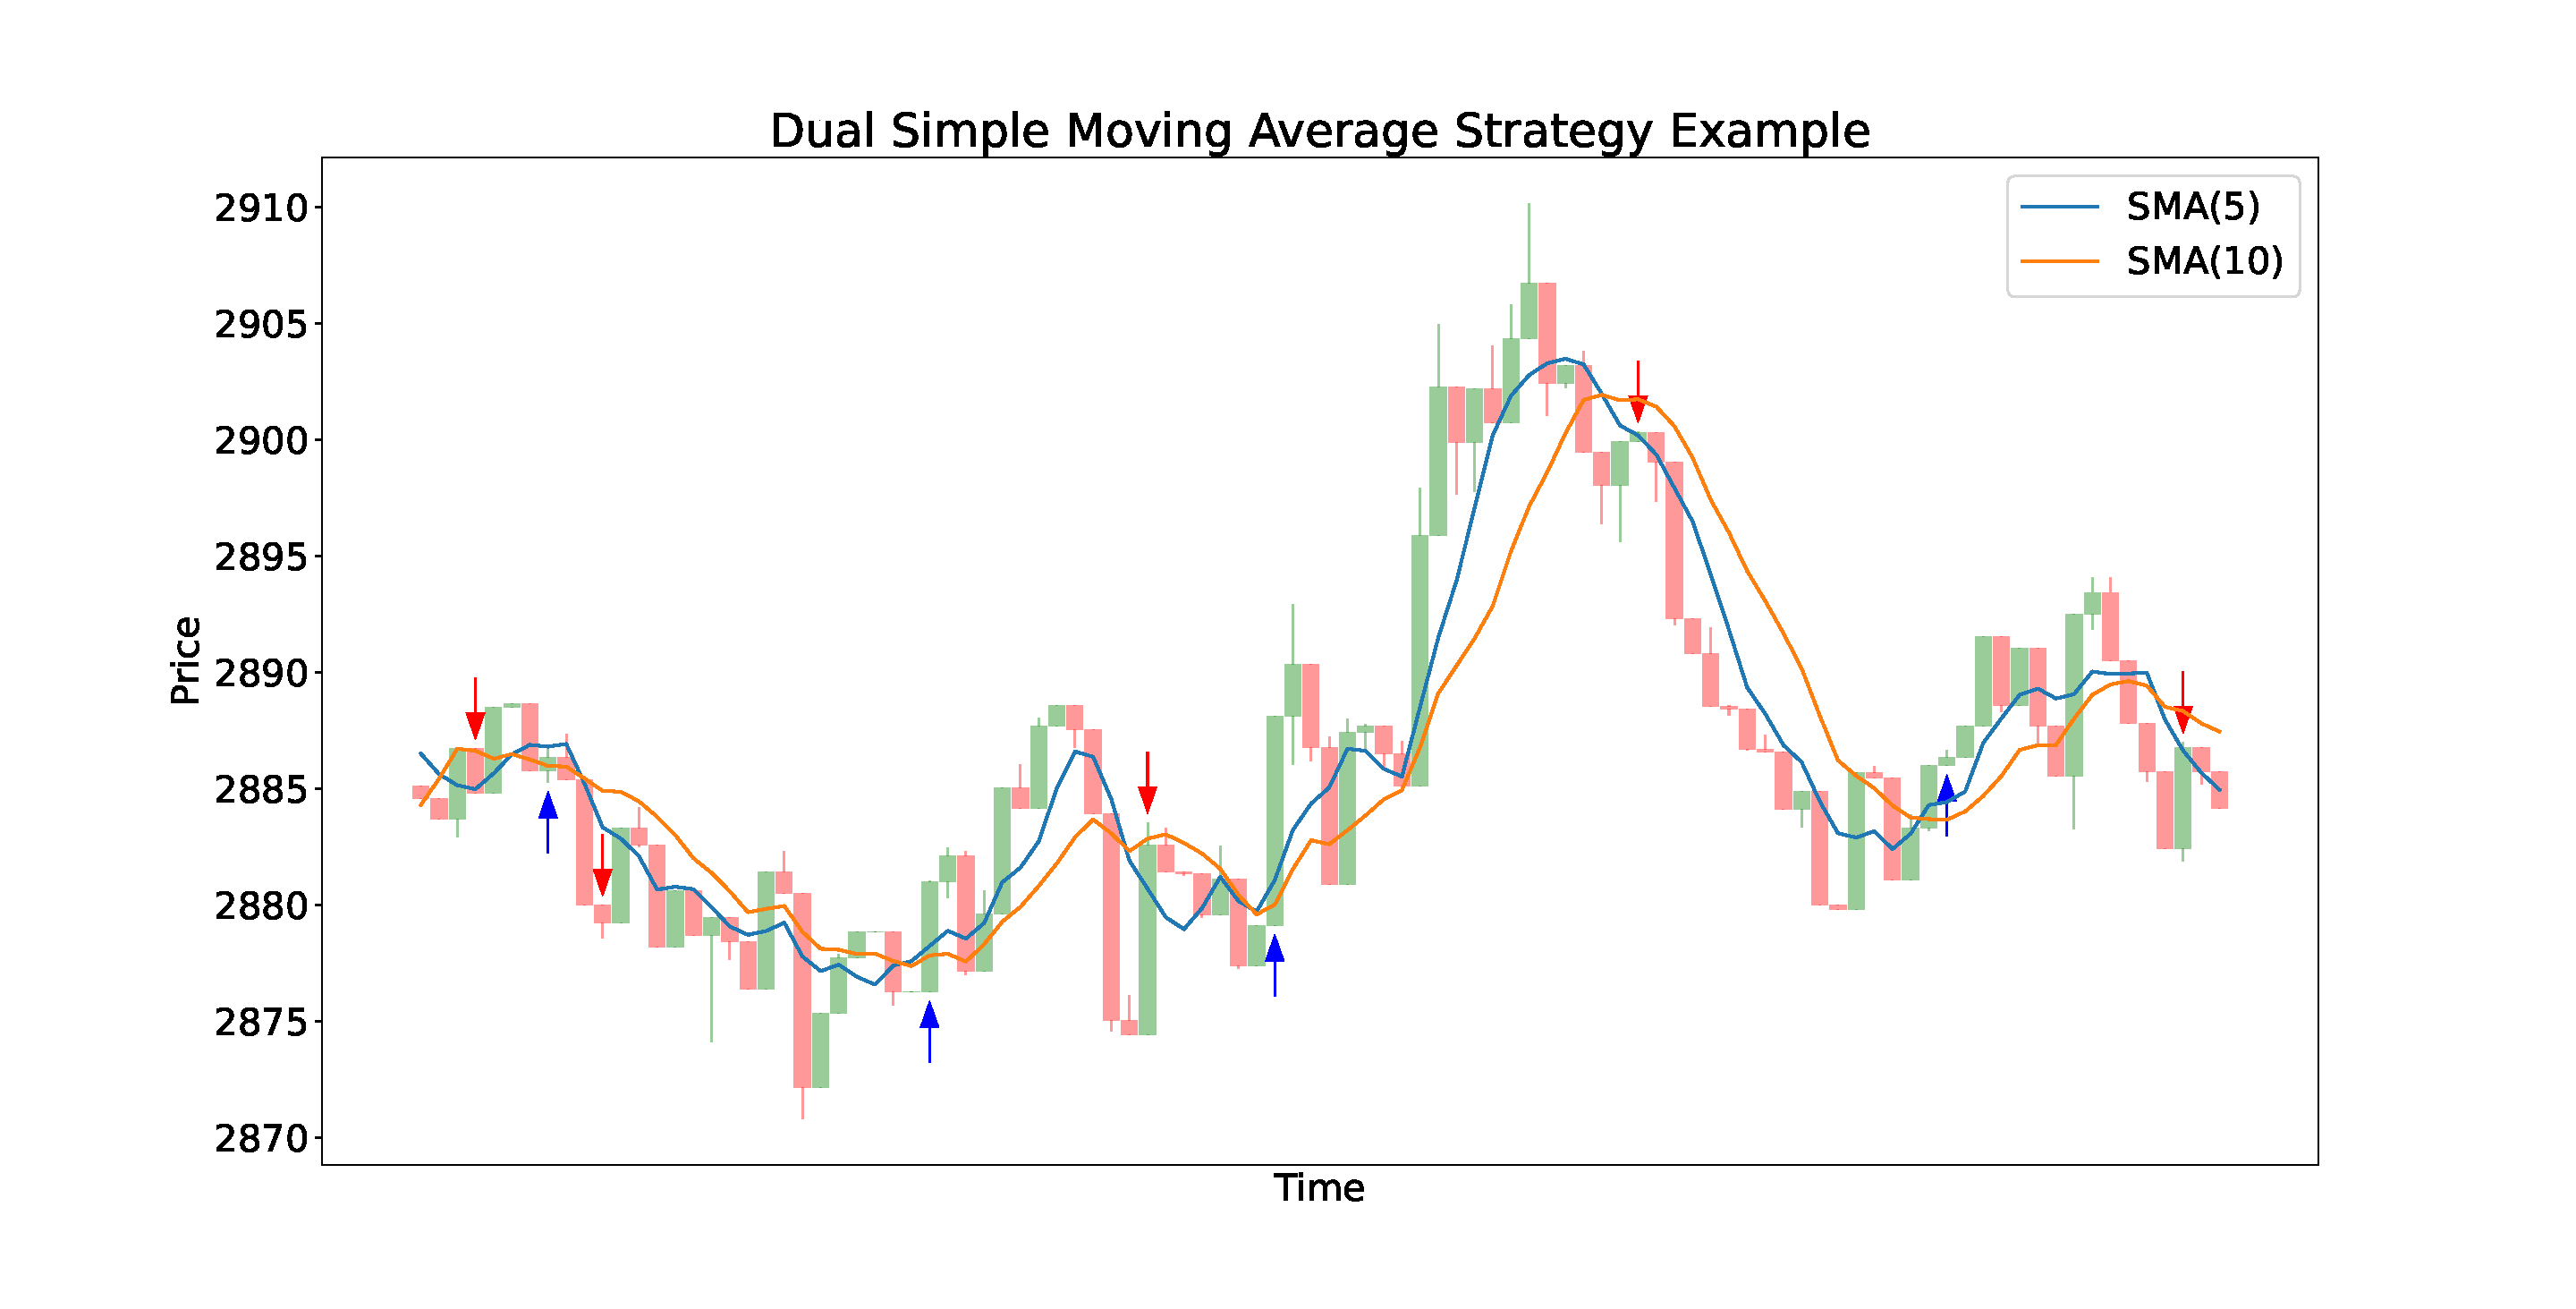
\includegraphics[width=\textwidth]{images/trading-strategies/sma-example}
    \caption{Dual Simple Moving Average Strategy Example}
    \label{fig:sma-example}
\end{figure}

\noindent
This strategy is very easy to understand and implement and can help to identify possible trend changes which generate entry and exit signals.
One of the greatest disadvantages is that the SMA is a lagging indicator and in quickly changing market conditions, the signals can be delayed.
Especially in sideways market regimes, the SMA's can cross often, which can lead to false signals \cite{sma-advantage-disadvantage}.
Here, the market regime recognition plays an important role.
Through this, the strategy can be disabled in sideways regimes and enabled if the market has a clear trend.

Often the criteria for stop-loss and take-profit levels are percentage and risk-reward ratio based, which means that the stop-loss has a fixed distance, e.g., 2\% and the take-profit is e.g. double the distance of the stop-loss distance (relative to the current price) \cite{sma-sl-tp}.
To achieve a more adaptive stop-loss and take-profit level determination, a self-developed mechanism called swing detection was added.

This detection finds swings in the price movements differs between swing high and swing low points.
A swing high point at time $t$ is a point where the closing price is greater than all closing prices in the intervall $[t-N; t+N]$.
Similarly, a swing low point is a point where the closing price is lower than all closing prices in the same intervall.
This allows detecting simple support and resistence zones, on which the stop-loss can be set.
Therefore, the strategy adapts to the current market behaviour.

%\autoref{fig:swing-high-low} shows syntetic price movements where at time $t=0$ swing highs are detected.

%TODO: Chart für swing highs und lows

The strategy has six parameters, consisting of the long-term and short-term SMA period, the order $N$ of the swing detection, which determines how significant the swing has to be, the maximum age of the last swing point, as well as a delta for the stop-loss and take-profit levels (identically to those in \autoref{chap:regression-ai-stategy}).
All parameter combinations where the short-term SMA period is greater than the long-term SMA period, have been filtered out and are not tested.

\begin{table}[H]
    \centering
    \begin{tabular}{L{4cm}ccc}
        \toprule
        \textbf{Parameter Name} & Min Value & Max Value & Step Size
        \\
        \midrule
        \textbf{Short-Term SMA Period} & 1   & 10    & 1    \\
        \textbf{Long-Term SMA Period}  & 2   & 20    & 1    \\
        \textbf{Swing Order $N$}       & 1   & 10    & 1    \\
        \textbf{Take-Profit Delta}     & 0.0 & 200.0 & 10.0 \\
        \textbf{Stop-Loss Delta}       & 0.0 & 100.0 & 10.0 \\
        \bottomrule
    \end{tabular}
    \caption{Dual Simple Moving Average Strategy Parameters}
    \label{tbl:sma-strategy-parameters}
\end{table}

\subsubsection{Triple Exponential Moving Average Strategy}

This strategy consists of three exponential moving averages (EMA) with different periods.
The shortest EMA identifies short-term trends, while the medium EMA identifies medium-term trends, and the long EMA identifies long-term trend.

The common application of the triple exponential moving average strategy generates a buy signal if the short-term EMA crosses above the medium-term EMA.
Additionally, the medium-term EMA must already be above the long-term EMA to validate the buy signal.
For sell signals, the short-term EMA must cross below the medium-term EMA and the medium-term EMA has to be bellow the long-term EMA \cite{ema3-basics}.

Therefore, the long-term EMA acts as a trend filter to reduce false positives mentioned in \autoref{chap:sma2}.
In this work, the long-term EMA is also used as a trend filter but not by its position relative to two other EMA's.
During the backtesting of the classic variant, it was noticed that many false entry signals were still generated, especially in sideways markets.
Therefore, the trend was filtered using a minimal slope of the long-term EMA.
The slope of the EMA is calculated by the slope of the regression line which is defined by the current EMA value (at time $t$) and the EMA value $i$ minutes in the past.

\[
    Slope = \frac{EMA_t - EMA_{t-i}}{i}
\]

\noindent
If the slope is greater than a predefined threshold, only long positions can be opened.
On the other hand, if the slope is less than the negated threshold, only short positions can be opened.
Otherwise, the strategy cannot open any new positions.

\autoref{fig:ema-example} shows the same synthetic price as in \autoref{fig:sma-example}.
Additionally, a third EMA with period 20 is added, which is used to calculate the slope.
The red-filled areas indicate zones where no positions can be opened.
So the entry signals in these areas are ignored.
In the green-filled areas, the entry signals are executed.

\begin{figure}[H]
    \centering
    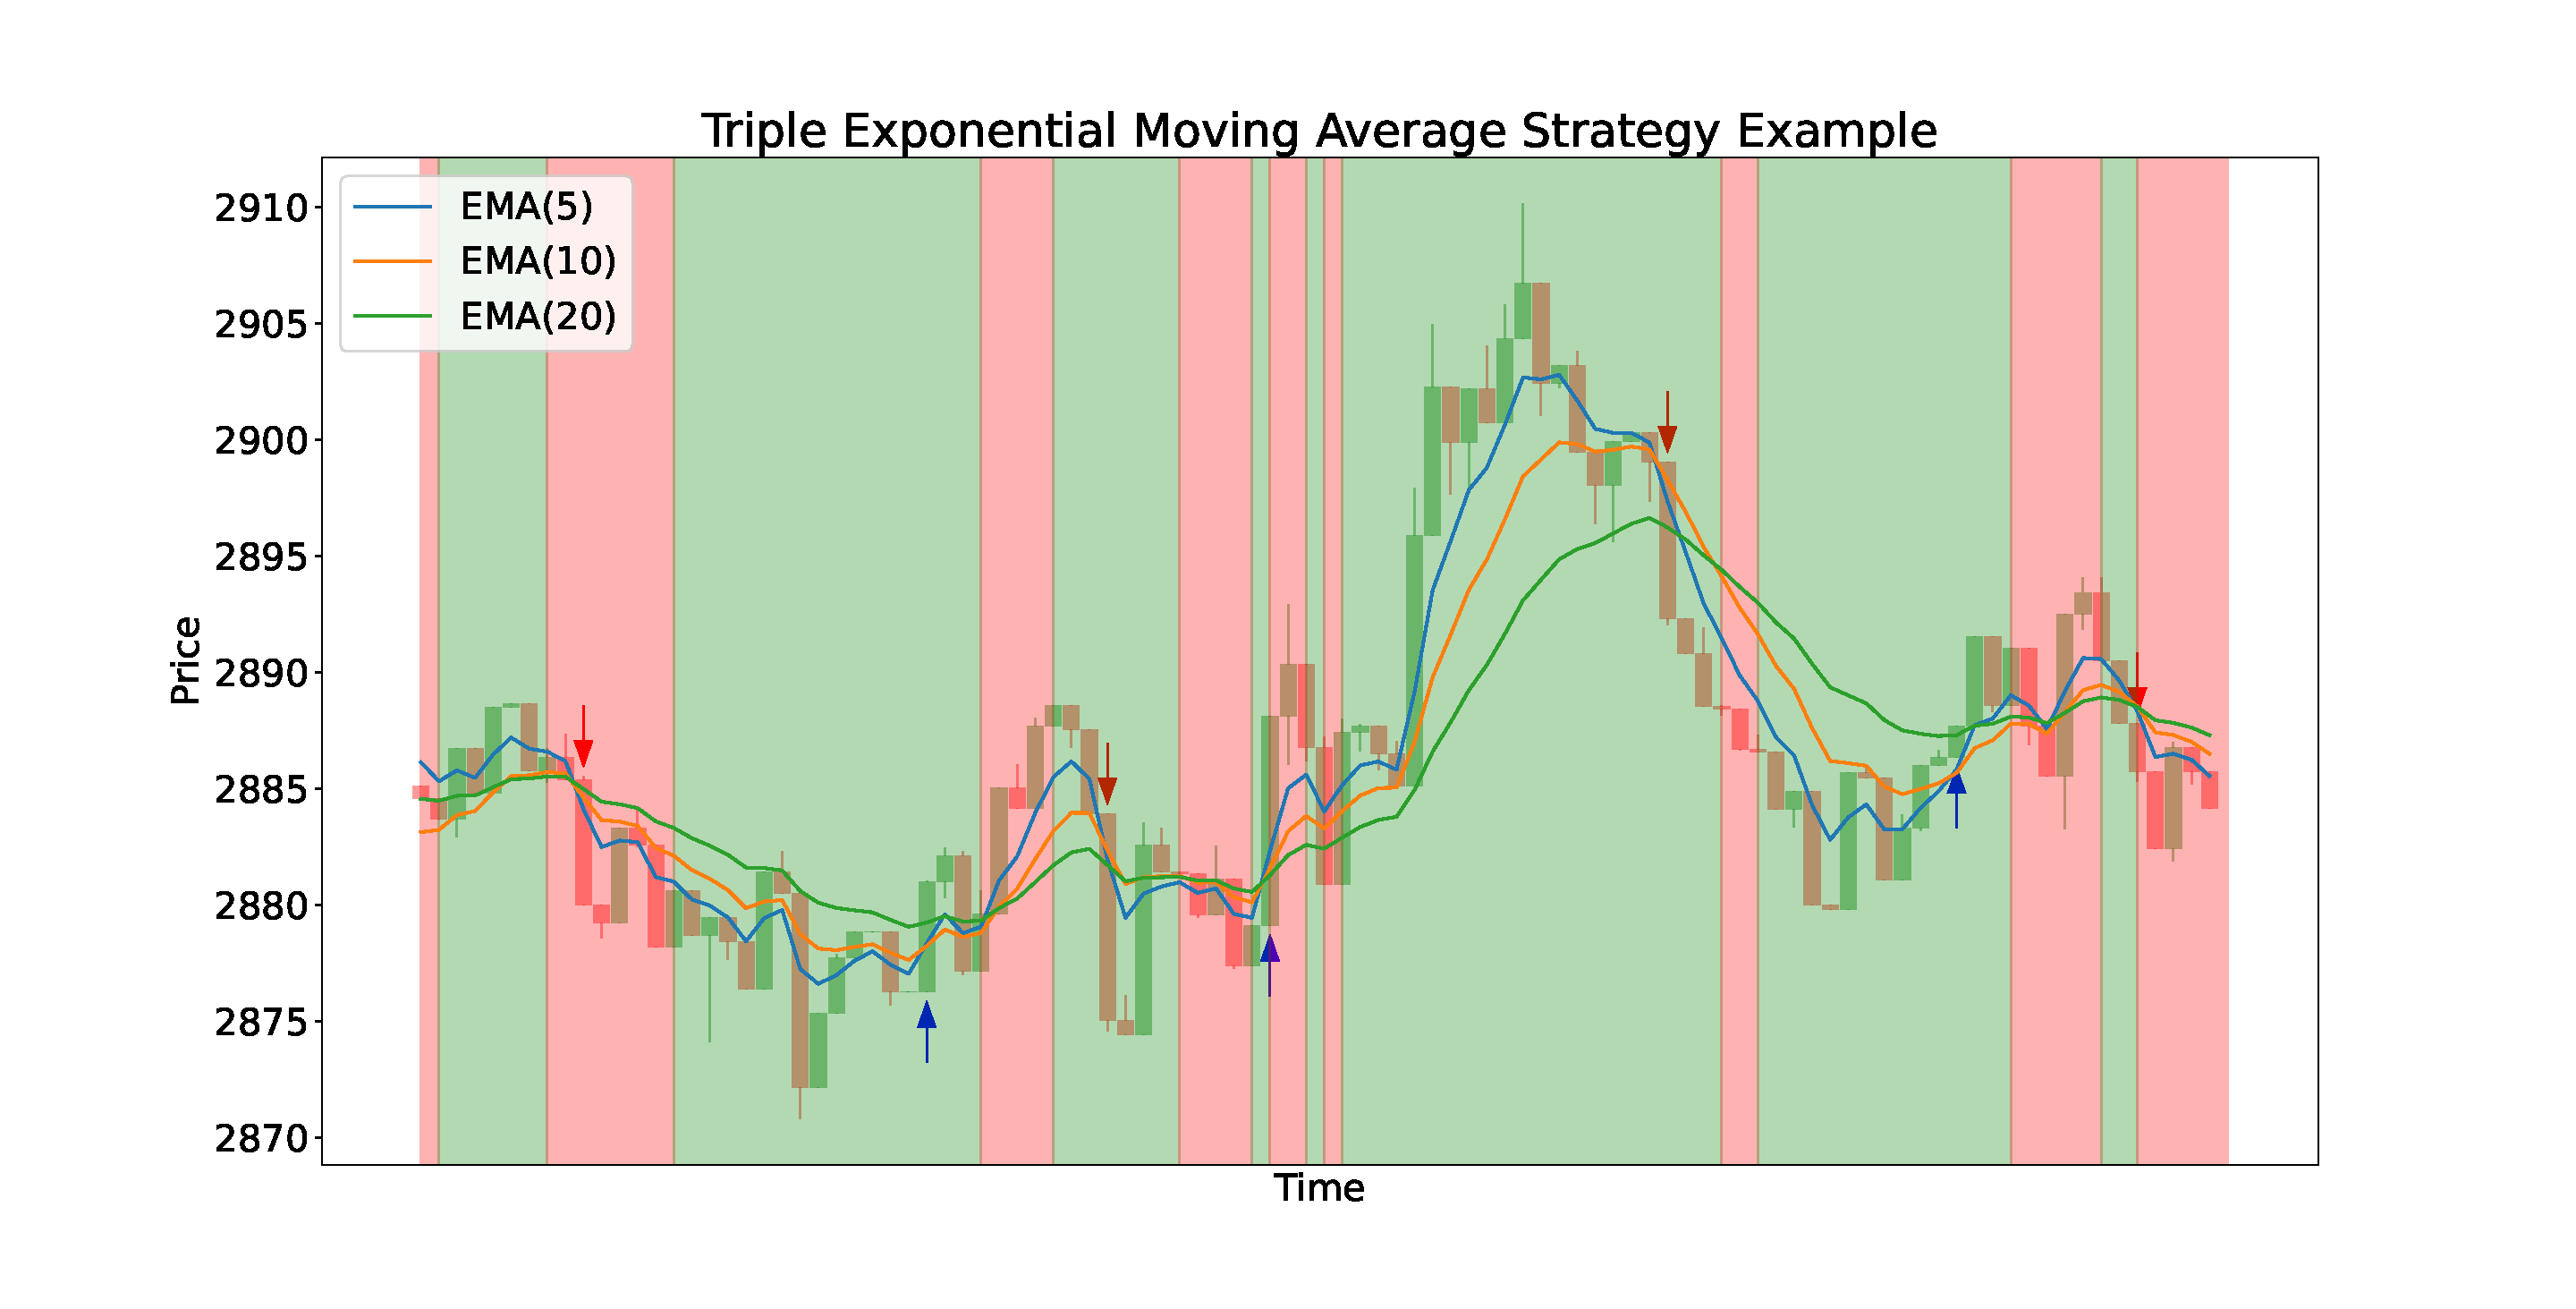
\includegraphics[width=\textwidth]{images/trading-strategies/ema-example}
    \caption{Triple Exponential Moving Average Strategy Example}
    \label{fig:ema-example}
\end{figure}

\noindent
In this strategy, the stop-loss and take-profit distance have been added as fixed parameters, which are also permuted.
All parameter combinations, where the short-term EMA period is greater than the medium-term EMA period, or the medium-term EMA period is greater than the long-term EMA period, are filtered out.

\begin{table}[H]
    \centering
    \begin{tabular}{L{4cm}ccc}
        \toprule
        \textbf{Parameter Name} & Min Value & Max Value & Step Size
        \\
        \midrule
        \textbf{Short-Term EMA Period}       & 3   & 10  & 2   \\
        \textbf{Medium-Term EMA Period}      & 5   & 30  & 3   \\
        \textbf{Long-Term EMA Period}        & 10  & 50  & 5   \\
        \textbf{Minimum EMA Slope}           & 0.2 & 1.2 & 0.2 \\
        \textbf{EMA Slope Window Length $i$} & 10  & 40  & 10  \\
        \textbf{Stop-Loss Distance}          & 10  & 100 & 10  \\
        \textbf{Take-Profit Distance}        & 10  & 150 & 10  \\
        \bottomrule
    \end{tabular}
    \caption{Triple Exponential Moving Average Strategy Parameters}
    \label{tbl:ema-strategy-parameters}
\end{table}

\subsubsection{Bollinger Bands Strategy}

The bollinger bands strategy is a mean reversion strategy, designed to exploit short-term price fluctuations.
This strategy assumes that after approaching or breaking through the outer bands, the price reverts to the central line (the moving average).
A buy entry signal is generated if a candle opens below the lower bollinger band and closes above the lower bollinger band.
This indicates a price reversal from an oversold condition.
On the other hand, a sell entry signal is generated if the candle opens above the upper bollinger band and closes below the upper bollinger band \cite{bb-basics}.

\autoref{fig:bb-example} shows the synthetic price, identically to \autoref{fig:sma-example} and \autoref{fig:ema-example}.
The blue-filled area shows the bollinger band, with the central line.

\begin{figure}[H]
    \centering
    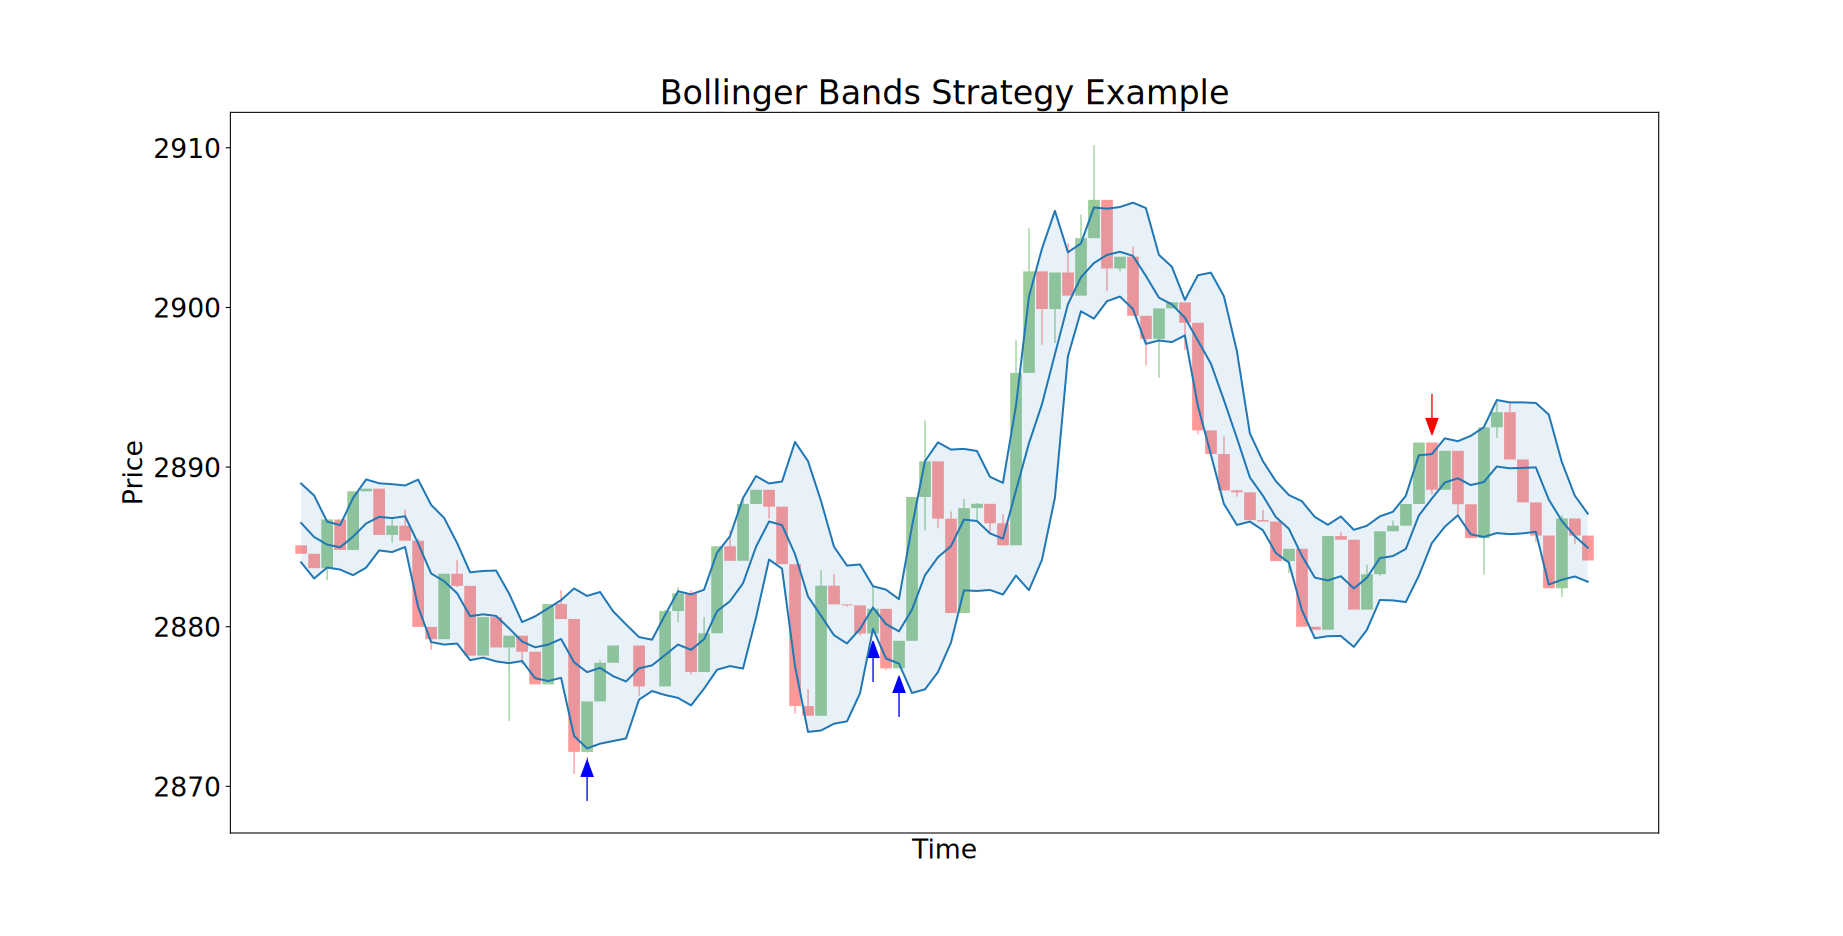
\includegraphics[width=\textwidth]{images/trading-strategies/bb-example}
    \caption{Bollinger Bands Strategy Example}
    \label{fig:bb-example}
\end{figure}

\noindent
The stop-loss level is set in a predefined distance relative to the current price.
The take-profit level is set at the level of the central line , with a certain delta being added (for buy signals) or subtracted (for sell signals) to the value of the middle line.

\begin{table}[H]
    \centering
    \begin{tabular}{L{4cm}ccc}
        \toprule
        \textbf{Parameter Name} & Min Value & Max Value & Step Size
        \\
        \midrule
        \textbf{Bollinger Band Period}      & 10   & 25    & 1    \\
        \textbf{No. of Standard Deviations} & 1.5  & 3.0   & 0.5  \\
        \textbf{Stop-Loss Distance}         & 10.0 & 100.0 & 20.0 \\
        \textbf{Take-Profit Delta}          & -5.0 & 20.0  & 2.0  \\
        \bottomrule
    \end{tabular}
    \caption{Bollinger Band Strategy Parameters}
    \label{tbl:bb-strategy-parameters}
\end{table}


    \newpage

    \section{Trading-Engine}
\label{chap:te}

For backtesting and live execution of trading strategies, a Java framework was built.
This chapter describes the use cases as well as the most important components of the trading engine.

\subsection{Use Cases of the Trading-Engine}
\label{chap:te-use-cases}

The developed trading engine represents a flexible and modular software platform that covers various use cases in the field of algorithmic trading.
The focus is on combining usability, adaptability, and performance.
The following are the most important use cases and features:

\begin{enumerate}
    \item \textbf{Backtesting trading strategies:} The trading engine enables the simulated execution of trading strategies on historical market data.
    This allows strategies to be tested under realistic conditions and their performance, robustness, and risk characteristics to be evaluated.
    By replicating historical market conditions, incorrect decisions can be identified early, and the trading strategy can be adjusted without using real capital.
    \item \textbf{Live execution in real-rime operation:} In addition to backtesting, the engine also supports real-time execution of strategies in the market.
    Through an interface to brokers, the engine can receive market data in real time, make trading decisions, and execute orders directly.
    This enables the engine to be used as the basis for automated trading in production environments.
    \item \textbf{Using money and risk management strategies:} An important use case is the implementation of different money and risk management approaches.
    Users can integrate various strategies for position sizing, stop-loss setting, or profit-taking, and examine their impact on strategy performance in backtests or in live operation.
    This supports the development of more stable and profitable trading approaches.
    \item \textbf{Connecting to any broker:} The trading engine is designed to connect to various brokers via interchangeable interfaces.
    This allows the engine to be combined with different trading systems and platforms.
    This flexibility enables its use in a wide variety of markets and infrastructures.
    \item \textbf{Development and integration of custom trading strategies:} A key feature of the engine is the ability for users to implement their own trading strategies.
    A clear separation between core functionality and strategy logic allows for flexible integration and testing of individual algorithms.
\end{enumerate}

\noindent
Most components of the trading engine are interchangeable and can be implemented by the user.
Only the core of the framework, including the fundamental process flow and control logic, remains fixed.
This allows users to tailor the engine to their individual needs, develop their own modules for data feeds, order management, strategy, or risk control, and thus ensure a high degree of flexibility in the use and further development of the platform.

\subsection{Architecture}

The trading engine consists of many modules ,which can be clustered into three main categories:

\begin{enumerate}
    \item Core Modules (Trading Engine)
    \item Applications
    \item Adapters
\end{enumerate}

\noindent
\autoref{fig:te-components} shows the components of the trading engine.

\begin{figure}[H]
    \centering
    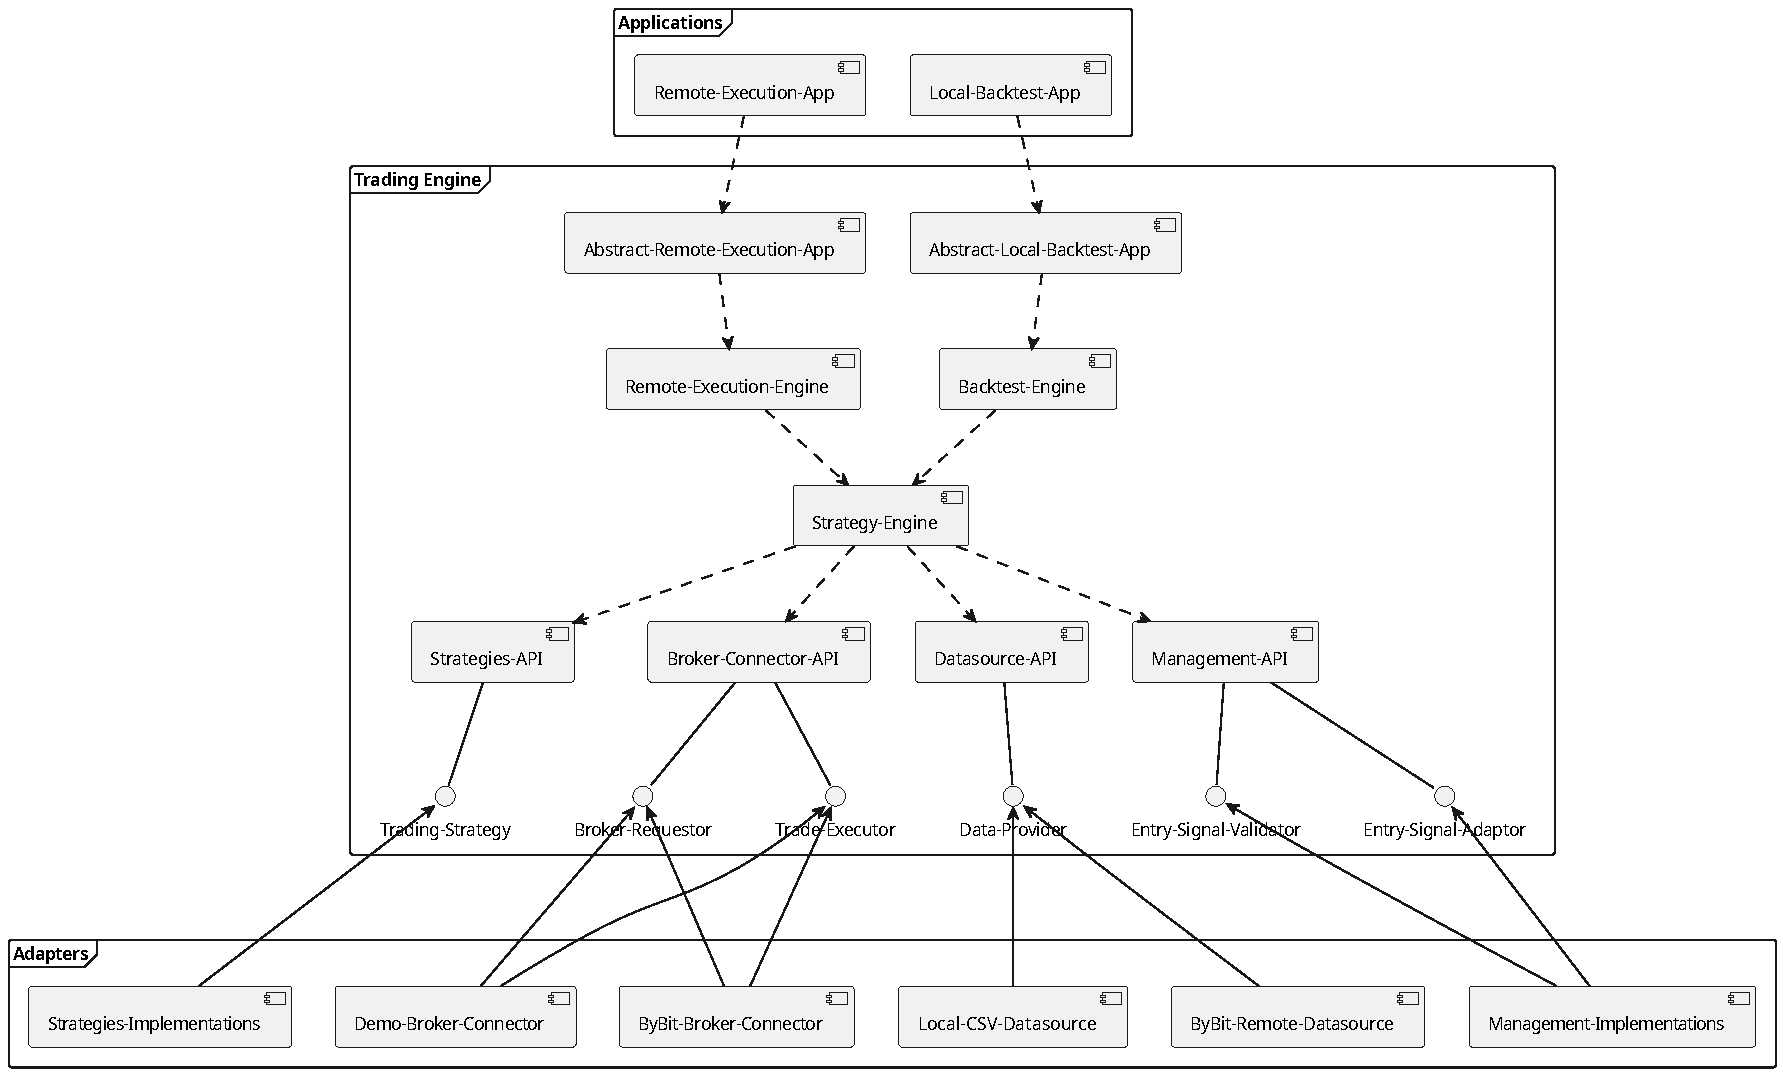
\includegraphics[width=\textwidth]{images/trading-engine/trading-engine-components}
    \caption{Trading Engine Components}
    \label{fig:te-components}
\end{figure}

\subsubsection{Plugin Architecture}

To achieve the flexibility mentioned in \autoref{chap:te-use-cases}, a plugin architecture was used.
Within the core, interfaces have been defined specifying which external functionalities are required (Service Provider Interface, or SPI).
To facilitate seamless interchangeability for users, the implementations of the interfaces in the external modules (Adapters) are loaded by the Java \texttt{java.util.ServiceLoader}.

The \texttt{ServiceLoader} loads classes at runtime that implement a specific interface or abstract class.
The classes to be loaded are specified via a configuration file in the \texttt{resources/}\\\texttt{META-INF/services} directory, which the \texttt{ServiceLoader} searches for in every JAR file in the classpath.
If a corresponding configuration file is found, the \texttt{ServiceLoader} can create an instance of the respective class using the default constructor \cite{java-service-loader}.

As an example, a Service Provider Interface for read access can be defined in a module named \texttt{spi}.

\lstinputlisting[language=Java, caption=SPI Definition, label=lst:service-loader-spi-definition, style=java]{java/trading-engine/service-loader-base.java}

\noindent
This interface can be implemented in multiple modules.
One implementation can be used to read data from files:

\lstinputlisting[language=Java, caption=File Repository Implementation, label=lst:service-loader-file, style=java]{java/trading-engine/service-loader-file.java}

\noindent
Here, a configuration file named \texttt{com.example.spi.read.ReadRepository} is located in the directory \texttt{resources/META-INF/services}.
This file contains the fully qualified class name of the implementation class (\texttt{com.example.adapter.file.read.}\texttt{FileReadRepository}).

\newpage
Another implementation can be used to read data from databases:

\lstinputlisting[language=Java, caption=Database Repository Implementation, label=lst:service-loader-db, style=java]{java/trading-engine/service-loader-db.java}

\noindent
Similar to the \texttt{FileReadRepository}, a file named \texttt{com.example.spi.read.ReadRepository} is located in the directory \texttt{resources/META-INF/services}.
However, this file contains \texttt{com.example.adapter.database.read.DatabaseReadRepository}.

The \texttt{ServiceLoader} searches in each JAR file in the classpath for files under \\\texttt{resources/META-INF/services} with the name \texttt{com.example.spi.read.}\texttt{ReadRepository} that contains the implementation of this interface, and creates them.

Since an external application has the ability to define the classpath, it can add or remove specific JARs.
This allows it to determine which implementations to use.
For example, it can decide to add only the \texttt{file-adapter} module or, if necessary, the \texttt{db-adapter} module if loading from a file, and a database simultaneously.

\subsubsection{Core Modules}

The core of the framework consists of several loosely coupled components that communicate with each other through well-defined APIs.
The most central unit is the \texttt{Strategy Engine} which contains the main logic for the execution of trading strategies, and controls the cooperation of the other subsystems.

The following components form the core:

\begin{enumerate}
    \item \textbf{Data Provider:} Obtains market data via a configurable \texttt{Datasource API}.
    The specific data source (local or remote) is integrated via adapters.
    \item \textbf{Trading Strategy:} The actual trading logic is integrated via the \texttt{Strategies API}.
    This API is separate from the framework and can be extended as required.
    \item \textbf{Broker Requestor \& Trade Executor:} Both communicate with brokers via a generic \texttt{Broker Connector API}, and enable both order placement and broker status queries, such as the current account balance or all open positions.
    \newpage
    \item \textbf{Entry Signal Adapter \& Entry Signal Validator:} These two components process and validate generated entry signals.
    They are linked to the \texttt{Management API} and enable additional risk checks, such as capital requirements or position limits.
    Currently, the implemented management includes all techniques introduced in \autoref{chap:risk-man} and is executed every time a strategy creates an entry signal.
\end{enumerate}

\noindent
Before the \texttt{Strategy Engine}, there are two other engines, named \texttt{Remote Execution}\\\texttt{Engine}, and \texttt{BacktestEngine}, which configure the \texttt{Strategy Engine}.
The difference between the engines is that the \texttt{Remote Execution Engine} defines the \texttt{Strategy Engine} asynchronously.
This means that a remote data source can stream market data via an API.
When new data arrives, the \texttt{Strategy Engine} is notified by the data source and starts executing the trading strategy.
For a local backtest, the \texttt{Strategy Engine} is configured so that data synchronization is handled by the \texttt{Backtest Engine}, not by the data source.

Abstract apps are modules that accept and parse user configurations.
For example, the task of the \texttt{Abstract Local Backtest App} is to ask the user via the console which strategy should be used for the backtest.
With the \texttt{Abstract Remote Execution App}, the configuration is not done via the console but primarily via environment variables.
The parsed configurations are then passed to the respective engines.

\subsubsection{Applications}

The application layer defines specific execution environments by defining the classpath with adapters.

\begin{enumerate}
    \item \textbf{Local-Backtest-App:} Executes trading strategies offline by using the \texttt{Local CSV }\\\texttt{Datasource} and the \texttt{Demo Broker Connector}.
    \item \textbf{Remote Execution App:} Executes strategies in real time and communicates with live broker interfaces.
\end{enumerate}

\noindent
Each application contains its own \texttt{main} method, which constructs and starts the respective implementation.

\subsection{Demo Broker}

For local backtests, the connection to a real broker must be mocked.
Therefore, the \texttt{Demo Broker Connector} is used to replace a real broker.
It takes over the main tasks including:

\begin{enumerate}
    \item \textbf{Order execution and position management:} Executing market, limit, take-profit, and stop-loss orders, including execution fee calculation.
    \item \textbf{Adapt trailing stop positions:} Monitoring trailing stop positions, and adapt the stop-level according to the most recent price.
    \item \textbf{Account balance management:} Managing the available account balance as well as the margin balance.
    \item \textbf{Store executed trades:} Storing the executed trades is essential for risk management and later analysis.
\end{enumerate}

\subsubsection{Order Execution and Position Management}

In the context of trading, order execution and position management are closely connected, because positions can be translated into three orders, where only two of them are actually executed.
As described in \autoref{chap:dealing-with-trading-fees}, it is necessary that the trading engine supports market and limit orders.
In real-life environments, most orders are not executed at the expected price, due to slippage \cite{ig-slippage}.
To simulate slippage, the trading engine can either use historical data of the underlying cryptocurrency, which is available in the lowest available timeframe (usually seconds or tick data), or simulate slippage randomly.
Two problems exist with simulations using historical data.
The first is that data in the seconds or tick range over a long period of time is difficult for private individuals to obtain.
Furthermore, latency must be simulated, which simulates the processing time and network traffic in live operation.
With random simulations, the problem arises that the backtest results are no longer deterministic.
Thus, a subsequent comparison of different strategies is subject to error.
For these reasons, the slippage factor is not taken into account during order execution.
This means that market orders are always executed at the most current available price, and limit orders are always executed at the specified order level.


\autoref{fig:te-position-opening} shows the process of opening a single position.
The margin in euro is calculated using the following formula \cite{margin-calculation}.


\[
    \text{Margin} = \frac{\text{Position Quantity}}{\text{Leverage} \cdot \text{Euro Conversion}} = \frac{\text{Position Size} \cdot \text{Open Price}}{\text{Leverage} \cdot \text{Euro Conversion}}
\]

\noindent
$\text{Euro Conversion}$ is the current price for converting the current counter currency into euros.
For example, for ETH/USDC the $\text{Euro Conversion}$ is the current price of EUR/USDC:
The conversion is done in euros because for different currency pairs with different counter currencies, the margin would be calculated in the respective counter currency.
For ETH/USDC, the margin is calculated in USDC according to the formula.
However, when trading ETH/BTC, the margin is calculated in BTC.
To obtain a result that is always in the same unit, or in this case, the same currency, the additional conversion is implemented.
It is important to note that it is also possible to implement conversion into any currency.
This way, the margin could also be calculated in BTC, for example.
Since USDC/EUR rates are offered by ByBit, it was easier in this case to compute historical data directly from ByBit and obtain the EUR/USDC rate through a conversion $\text{EUR/USDC} = \frac{1}{\text{USDC/EUR}}$.

\begin{figure}[H]
    \centering
    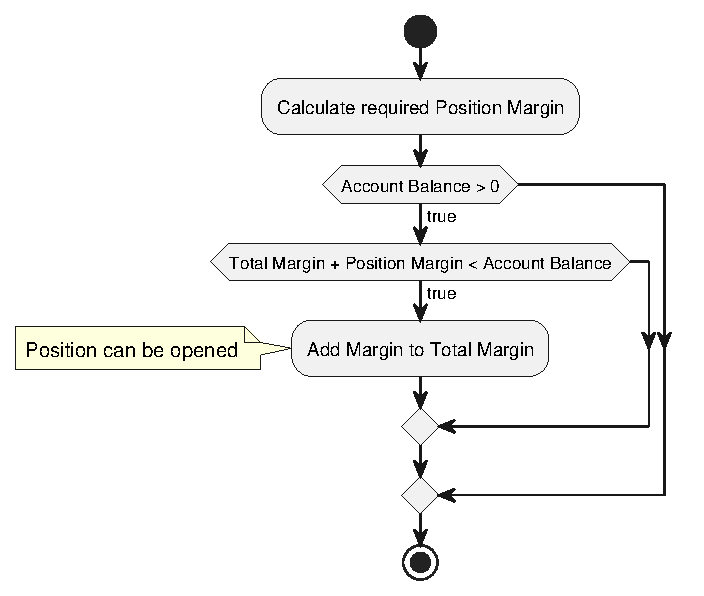
\includegraphics[width=0.7\textwidth]{images/trading-engine/position-opening}
    \caption{Opening a Single Position}
    \label{fig:te-position-opening}
\end{figure}

\noindent
After a position has been opened, it must be closed again at a later point in time.
This can happen either by reaching the stop loss or take profit, or by intentionally closing it, which is controlled by a strategy.
\autoref{fig:te-position-closing} shows the process of closing a single position.
The profit in euro is calculated using the following formula \cite{margin-calculation}:

\[
    \text{Profit} = \frac{(\text{Close Price} - \text{Open Price}) * \text{Position Size}}{\text{Euro Conversion}} *
    \begin{cases}
        -1,& \text{if Sell-Position}\\
        1,              & \text{otherwise}
    \end{cases}
\]

\noindent
Just like with the margin calculation, a conversion into euros also takes place, so that when trading on different pairs with different counter currencies at the same time, the profit is always calculated in the same unit.

\begin{figure}[H]
    \centering
    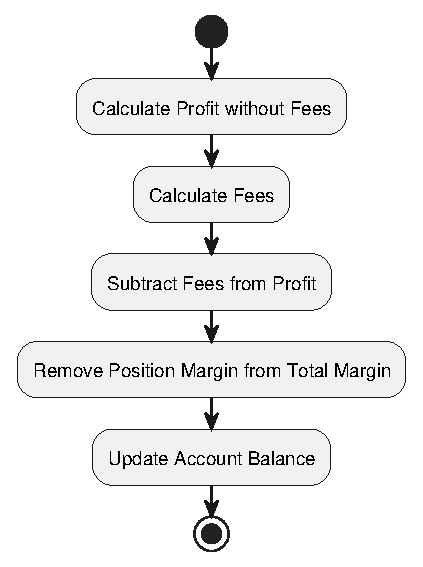
\includegraphics[width=0.4\textwidth]{images/trading-engine/position-closing}
    \caption{Closing a Position}
    \label{fig:te-position-closing}
\end{figure}

\noindent
If there are already positions in a market, the process for opening a new position must be extended.
This is because the size of the open positions must first be reduced, and then a new position (smaller than the original) must be opened.
This is comparable to a netting process.
\autoref{fig:te-complete-position-opening} shows the process of opening a position taking into account that other open positions can already exist.

If a strategy is designed in such a way that all positions in the opposite direction should first be closed when a signal is given in one direction, the strategy must first send an exit signal before the entry signal, which closes all other positions


\begin{figure}[H]
    \centering
    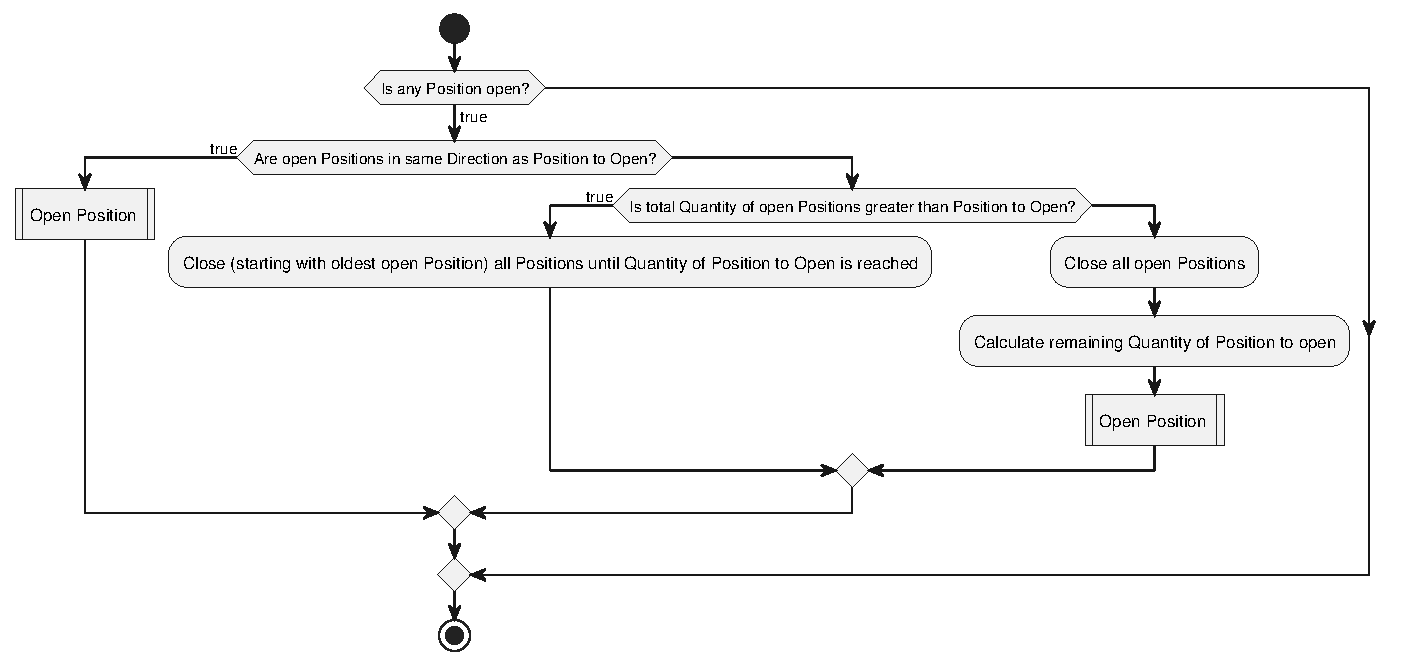
\includegraphics[width=\textwidth]{images/trading-engine/complete-position-opening}
    \caption{Opening a Position}
    \label{fig:te-complete-position-opening}
\end{figure}

\subsubsection{Adapting Trailing Stop Positions}

Trailing stop positions are positions with a dynamic stop order.
The stop level moves automatically with the price as soon as it moves in the desired direction.
For a buy position, the stop level moves if the price rises.
If the price falls, the stop remains unchanged \cite{ig-trailing}.

\autoref{fig:trailing-stop} shows a synthetic closing price (black) and a trailing-stop order with 60 points distance (red) for a buy position.
In the green-filled areas, the price moves in the desired direction, so the trailing-stop level follows the price.
In the red-filled areas, the prices do not move in the desired direction, so the trailing-stop level does not move.
An exception is the red-filled area after $t=3$, where the price moves in the desired direction, but the trailing stop does not.
This is because there is not yet a 60-point gap between the price and the stop level.
Therefore, the stop only moves again once the 60-point gap is restored.

\begin{figure}[H]
    \centering
    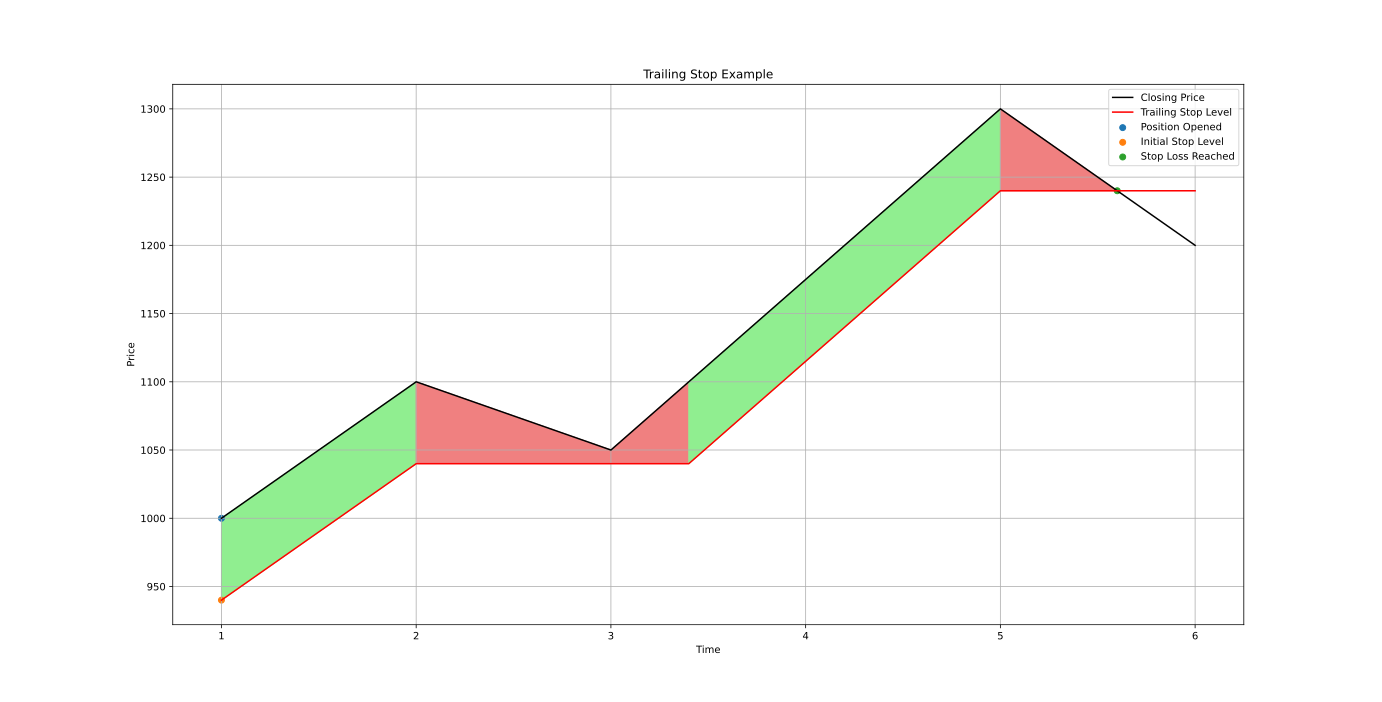
\includegraphics[width=\textwidth]{images/trading-engine/trailing-stop}
    \caption{Trailing Stop Example}
    \label{fig:trailing-stop}
\end{figure}


    \newpage

    \section{Backtesting Trading Strategies}
\label{chap:backtesting}

The quantitative evaluation of trading strategies requires a structured and comprehensible testing environment which was introduced in \autoref{chap:te}.
This chapter describes the executed backtests, which aim to verify the performance of the develop trading strategies in \autoref{chap:trading-strategies} under realistic conditions.

Backtesting describes a performance simulation of a trading strategy based on historical data.
This involves investigating how a specific strategy would have performed in the past if it had been executed under the given market conditions.
The goal is to gain initial insights into the robustness, profitability, and risk profile of the approach before it is used in live trading \cite{backtesting}.

\subsection{Trading Strategy Parameter Selection}

In contrast to the classic machine learning process, the parameter selection for the ultimately executed strategies is performed without the training set.
This also applies to strategies that use deep learning (\autoref{chap:ai-strategies}).
Unlike the training of deep learning models, which learn from the training data and adapt their internal states based on the training data, the trading strategies are initialized with fixed parameters.
This corresponds to the fitting of deep learning models.
However, the subsequent process is identical.
The strategies are validated with their previously defined parameters on the validation set to find the best possible parameters.

\subsection{Executing Backtests}

Due to the large number of parameter combinations shown in \autoref{tbl:parameters-number}, backtesting all combinations is not possible due to the execution time.
Therefore, only 1000 combinations per strategy were tested on the validation set.
In order to cover the greatest possible variance of the parameters, the combinations were not sampled randomly from the set of all possible combinations, but the combinations were sorted in lexicographic order and sampled at constant intervals.

\begin{table}[H]
    \centering
    \begin{tabular}{L{8cm}c}
        \toprule
        Strategy Name & Number of Parameters
        \\
        \midrule
        \textbf{Regression AI Strategy}                     & 8,820     \\
        \textbf{Classification AI Strategy}                 & 5,600     \\
        \textbf{Dual Simple Moving Average Strategy}        & 98,000    \\
        \textbf{Triple Exponential Moving Average Strategy} & 1,555,200 \\
        \textbf{Bollinger Bands Strategy}                   & 8,320     \\
        \bottomrule
    \end{tabular}
    \caption{Number of Parameters per Strategy}
    \label{tbl:parameters-number}
\end{table}

\subsection{Evaluating Backtests}

Due to the length, the detailed results of the backtests \footnote{Detailed results in \autoref{chap:strategy-results-on-validation-data}}, including the parameters \footnote{Detailed parameters per strategy and regime in \autoref{chap:best-strategy-parameters}} that led to the respective results, can be found in the appendix.
Here, only the results of the strategies with the highest cumulative last equity combined across all market regimes are presented.

\begin{table}[H]
    \centering
\begin{tabular}{ll|cccc}
    \toprule
    \multicolumn{2}{r|}{Strategy} & \begin{tabular}[c]{@{}c@{}}
                                        Classification\\AI
    \end{tabular} & Dual SMA & Triple EMA & \begin{tabular}[c]{@{}c@{}}
                                                Bollinger\\Bands
    \end{tabular} \\
    \midrule
    \multicolumn{2}{l|}{\textbf{Number of Trades}} & 267 & 3473 & 870 & 275 \\
    \multicolumn{2}{l|}{\textbf{Maximum Gain}} & 956 & 357 & 875 & 191 \\
    \multicolumn{2}{l|}{\textbf{Maximum Loss}} & -245 & -160 & -135 & -64 \\
    \multicolumn{2}{l|}{\textbf{Profits Std.}} & 280 & 37 & 105 & 41 \\
    \multirow{3}{*}{\textbf{Equity}} & \textbf{Minimum} & -2404 & -23   & -75   & 49   \\
    & \textbf{Maximum} & 57908 & 15510 & 10717 & 2510 \\
    & \textbf{Last}    & 55567 & 15159 & 9502  & 2510 \\
    \multicolumn{2}{l|}{\textbf{Maximum Drawdown}} & 4 & 149 & 126 & 51 \\
    \multicolumn{2}{l|}{\textbf{Win Ratio}} & 64 & 49 & 33 & 42 \\
    \bottomrule
\end{tabular}

    \caption{Combined Strategy Results}
    \label{tbl:combined-strategy-results}
\end{table}

\noindent
As seen in \autoref{tbl:combined-strategy-results} the Classification AI strategy achieves by far the best cumulative results on the validation set, with the lowest maximum drawdown and the highest win ratio.
But on the other hand, it also has the greatest loss.

To compare the out-of-sample performance \footnote{Detailed out-of-sample results in \autoref{chap:oos-strategy-results}}, all strategies have also been tested with the best parameters on the validation set on the backtest set.

\begin{table}[H]
    \centering
\begin{tabular}{ll|cccc}
    \toprule
    \multicolumn{2}{r|}{Strategy} & \begin{tabular}[c]{@{}c@{}}
                                        Classification\\AI
    \end{tabular} & Dual SMA & Triple EMA & \begin{tabular}[c]{@{}c@{}}
                                                Bollinger\\Bands
    \end{tabular} \\
    \midrule
    \multicolumn{2}{l|}{Number of Trades} & 173 & 5494 & 553 & 444 \\
    \multicolumn{2}{l|}{Maximum Gain} & 424 & 268 & 937 & 163 \\
    \multicolumn{2}{l|}{Maximum Loss} & -144 & -63 & -207 & -88 \\
    \multicolumn{2}{l|}{Profits Std.} & 92 & 9 & 179 & 32 \\
    \multirow{3}{*}{Equity} & Minimum & -2630 & -4694 & -948 & -4378 \\
    & Maximum & 2630  & 0     & 4048 & 0     \\
    & Last    & -2630 & -4694 & 560  & -4365 \\
    \multicolumn{2}{l|}{Maximum Drawdown} & 200 & 898314 & 131 & 87 \\
    \multicolumn{2}{l|}{Win Ratio} & 23 & 26 & 19 & 25 \\
    \bottomrule
\end{tabular}

    \caption{Combined Out-of-Sample Strytegy Results}
    \label{tbl:combined-strategy-results-oof}
\end{table}


\noindent
\autoref{tbl:combined-strategy-results-oof} shows that the strategies have a poor out-of-sample performance, resulting in either high losses or very volatile equity curves, which are not useful for real live trading.
This shows that there is also a kind of overfitting in the parameter selection.
While the strategies work well on the validation data, they fail in the out-of-sample tests.

\subsection{Fee-Impacts}

A key component of the realistic evaluation of algorithmic trading strategies is the consideration of transaction costs.
These costs can have a significant impact on performance depending on trading frequency, broker model, and market conditions.

In this study, trading fees were integrated directly into the trading engine so that they are automatically considered with every order execution in backtesting.
The chosen model is based on the ByBit fee structure based on the traded volume (0.02\% for maker orders and 0.055\% for taker orders).
This enables realistic backtests of trading strategies.
However, things like slippage were not taken into account but can be added in later improvements.

\autoref{tbl:fees} shows the sum of all fees incurred with the best parameters on the validation data (In-Sample) and on the test data (Out-of-Sample).

\begin{table}[H]
    \centering
    \centering
    \begin{tabular}{l|ccc}
        \toprule
        \multirow{2}{*}{\textbf{Strategy}} & \multicolumn{2}{c}{In-Sample} & Out-of-Sample \\
        & Total Fees & Relative to PnL & Total Fees \\
        \midrule
        \textbf{Classification AI} & 3570       & 6.4\%           & 1937       \\
        \textbf{Dual SMA}          & 4219       & 27.8\%          & 2874       \\
        \textbf{Triple EMA}        & 3858       & 40.6\%          & 4652       \\
        \textbf{Bollinger Bands}   & 1127       & 44.9\%          & 1858       \\
        \bottomrule
    \end{tabular}
    \label{tbl:fees}
    \caption{Total Trading Fees}
\end{table}

\noindent
It becomes clear that a considerable amount of fees is incurred, which amounts to up to approximately 40\% of the net profit (Triple EMA).
However, when comparing the number of trades across strategies, an interesting insight emerges.
As shown in \autoref{tbl:combined-strategy-results}, the Dual SMA strategy executes by far the most trades (3473 in total) on the validation set, but despite this high trading frequency, its relative fee impact is noticeable lower compared to the Triple EMA strategy, which executed only 870 trades.
This indicates that not only the number of trades but also entry and exit timing, holding duration, and trade efficiency play a crucial role in determining fee sensitivity.

This highlights that fee efficiency is not strictly a function of trading frequency alone.
While one might intuitively expect more trades to always lead to higher costs, the Dual SMA strategy demonstrated that a high-frequency system can still be cost-efficient if implemented with consistent execution logic and stable market conditions.

Most importantly, these findings emphasize the critical importance of incorporating fees in every phase of strategy evaluation.
Conducting backtests without fees would draw an overly optimistic and misleading picture of strategy performance.
For instance, a strategy that appears profitable on a gross level may become unprofitable once realistic costs are accounted for.

For this reason, no backtests or performance evaluation in this work was conducted without accounting for trading fees.
All strategies were tested under the assumption of realistic maker and taker fees, according to the selected broker ByBit.
This ensures that every performance metric presented reflects realistic scenarios and therefore increases the practial relevance and robustness of the results.



    \newpage

    \section{Stress Testing}

    \newpage

    \section{Live Testing}
\label{chap:live-test}

Despite the poor results from \autoref{chap:backtesting}, a strategy will be executed live on a demo account at ByBit for further development.
The primary purpose of this live test is not to achieve profitability but rather to validate the end-to-end functionality of the trading infrastructure under realistic market conditions.


\subsection{Broker Setup}

To connect to ByBit, the \texttt{ByBit Broker Connector} and \texttt{ByBit Remote DataSource} components have been used.

The \texttt{ByBit Remote DataSource} is able to:

\begin{enumerate}
    \item Request historical market data via the ByBit \texttt{Get Kline} API endpoint \cite{get-kline}.
    \item Stream market data through the ByBit \texttt{Kline} websocket endpoint \cite{stream-kline}.
\end{enumerate}

\noindent
The \texttt{ByBit Broker Connector} is able to execute the following actions via the ByBit API:

\begin{enumerate}
    \item Request the current wallet balance as well as the current margin \cite{wallet-balance}.
    \item Place orders in the market, which include open, take-profit, and stop-loss orders.
    Each Order is supported as limit and market order \cite{place-order}.
    \item Request all open positions for one or multiple pairs \cite{position-info}.
    In this paper, this only includes positions on \ethusdc.
    \item Request closed trades within a specified time period \cite{closed-pnl}.
\end{enumerate}

\noindent
The connection to ByBit is established by an API key and an API secret, which can be created in the ByBit web interface.
The distinction between a demo account and a real money account is regulated by ByBit via the base URL, which differs in each case.
To use the demo account, for REST endpoints, the base url \texttt{https://api-testnet.bybit.com} must be used.
For the real money account, the base url \texttt{https://api.bybit.com} must be used \cite{integration}.
To stream the market data, no distinction is required because the base URL \texttt{wss://stream.bybit.com/v5/public/linear} \cite{ws-connect} for streaming USDC market data is a public endpoint that can be used without an API Key.
In the trading engine, the base URLs, API key, and API secret are set via environment variables to achieve an independent implementation, configured by the user.

\subsection{Live-Test Results}

Using the trading engine configuration described above, a live execution of the triple exponential moving average strategy was performed from \liveStartDataStartDate~to \liveStartDataEndDate.
To keep the environment as similar as possible to the local backtest environment, the balance of the demo account was set to 5000 USDC at startup.

\begin{table}
    \centering
    \centering
\begin{tabular}{ll|c}
    \toprule
    \multicolumn{2}{l|}{Strategy} & Triple EMA \\
    \midrule
    \multicolumn{2}{l|}{\textbf{Number of Trades}} & 66 \\
    \multicolumn{2}{l|}{\textbf{Maximum Gain}} & 304 \\
    \multicolumn{2}{l|}{\textbf{Maximum Loss}} & -228 \\
    \multicolumn{2}{l|}{\textbf{Profits Std.}} & 82 \\
    \multirow{3}{*}{\textbf{Equity}} & \textbf{Minimum} & 3640 \\
    & \textbf{Maximum} & 5000 \\
    & \textbf{Last}    & 3913 \\
    \multicolumn{2}{l|}{\textbf{Maximum Drawdown}} & 27 \\
    \multicolumn{2}{l|}{\textbf{Win Ratio}} & 27 \\
    \bottomrule
\end{tabular}

    \caption{Live-Test Statistics}
    \label{tbl:live-results}
\end{table}

\begin{figure}[H]
    \centering
    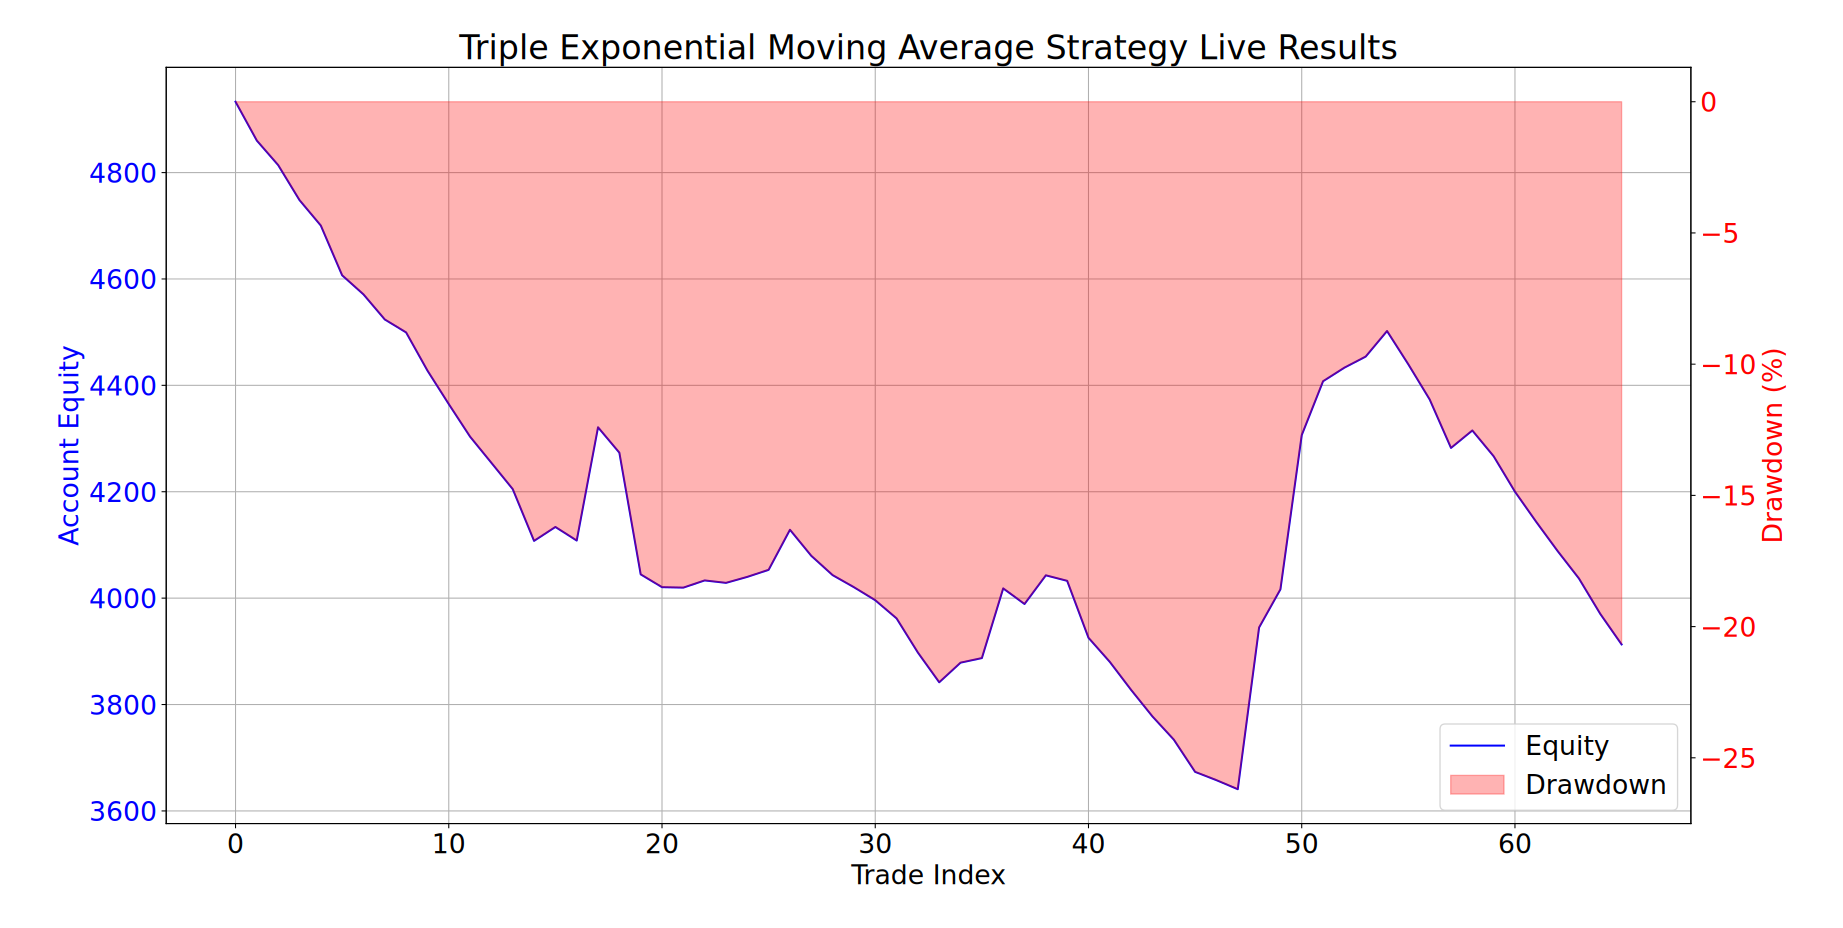
\includegraphics[width=\textwidth]{images/live/live-result}
    \caption{Live-Test Results}
    \label{fig:live-results}
\end{figure}

\noindent
As \autoref{tbl:live-results} and \autoref{fig:live-results} show, the strategy does not deliver profitable results in the live test either.

The logs \footnote{The logs are not published in this work due to their length.} show that the connection (data streaming) was interrupted several times during execution by the broker or due to network problems.
In these cases, the trading engine attempts to reconnect every ten seconds.
As soon as the connection is re-established, the engine continues to run normally.
The only limitation is that the internal state of the currently executing strategies is not reset, as this function does not yet exist.
This is particularly relevant if a connection interruption causes several candles to be skipped, making it appear to the strategies as if there were a jump in the data.
A mechanism must therefore be built in that detects gaps in the data and resets the strategies.
In the test carried out, however, this did not pose a problem, as the connection interruptions never lasted longer than a few seconds and no candles were missed.


    \newpage

    \section{Conclusion}

\subsection{Key Findings}


\section{Aim of further Works}



% ====================  Listings  ======================


    \newpage


    \section{References}
    \printbibliography[title=~]


\end{document}
